This chapter explores the results of performing the BANFF fit using
the $\pod$-only samples. We have confirmed that the fit machinery
is working and that the samples demonstrate sensitivity to flux and
cross section parameters. The focus in this chapter is to examine
the results of the $\pod$-only data fit and compare it against the
FGD-only result.

The chapter will proceed in the following order. First, since we have
remained purposefully blind up to this state in the analysis, the
data will be examined in \prettyref{sec:Prefit-Sample-Distributions}.
Next the postfit results will be carefully examined and compared with
that of the FGD-only fit in \prettyref{sec:Postfit-Results}. Finally,
a chapter summary is provided in \prettyref{sec:ResultsSummary}.


\section{Prefit Sample Distributions\label{sec:Prefit-Sample-Distributions}}

This section presents the first look at the data for the 12 samples
according to the fit bins set in \prettyref{chap:P0DinBANFF}. The
samples are categorized into four true interaction modes as described
earlier: $\nu$ CCQE, $\nu$ non-CCQE, $\antinu$ CCQE, and $\antinu$
non-CCQE. However, true fiducial volume (FV) and out of FV events
are not differentiated in this case. The prefit samples with the data
shown are presented between \prettyref{fig:Data-and-prefit-wtr-numu1Trk}
and \prettyref{fig:Data-and-prefit-air-numuRHCNTrks}. First the water-in
samples are displayed, and then the water-out samples are shown. As
we saw before, the water-in and water-out samples are qualitatively
the same.

In general, we notice good agreement between the data and prefit distributions.
Their agreement is represented in one-dimensional profiles with the
data to prefit ratio shown below the histograms. Evidence of the $\pod$
bulging effect in the most downstream layers can be seen in all water-in
samples. In particular, since there is more true mass in the most
downstream layers, particles with lower momenta are more likely to
enter the TPC than predicted by the MC using the as-built mass. Better
agreement is observed in the water-out periods, but there is some
data tension.

\begin{figure}
\begin{centering}
\subfloat[Momentum in MeV/c]{\begin{centering}
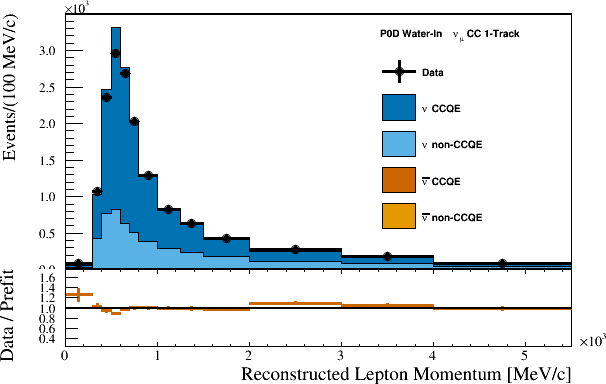
\includegraphics[width=0.48\textwidth]{Chapters/Figures/FitterResults/Prefit/png/P0D_Water_NuMu_CC1Track_mumom_rxn_prefit}
\par\end{centering}
}\subfloat[$\cos\theta$]{\begin{centering}
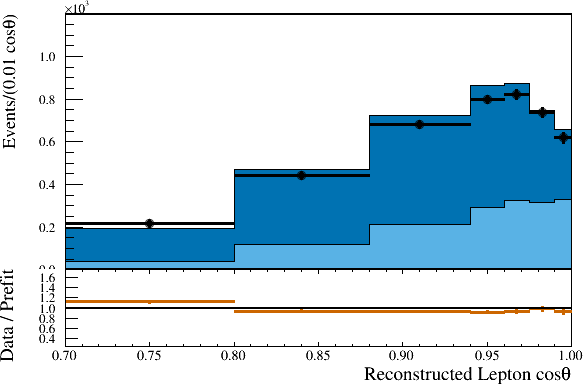
\includegraphics[width=0.48\textwidth]{Chapters/Figures/FitterResults/Prefit/png/P0D_Water_NuMu_CC1Track_mucostheta_rxn_prefit}
\par\end{centering}
}
\par\end{centering}
\begin{centering}
\subfloat[Momentum-$\cos\theta$]{\begin{centering}
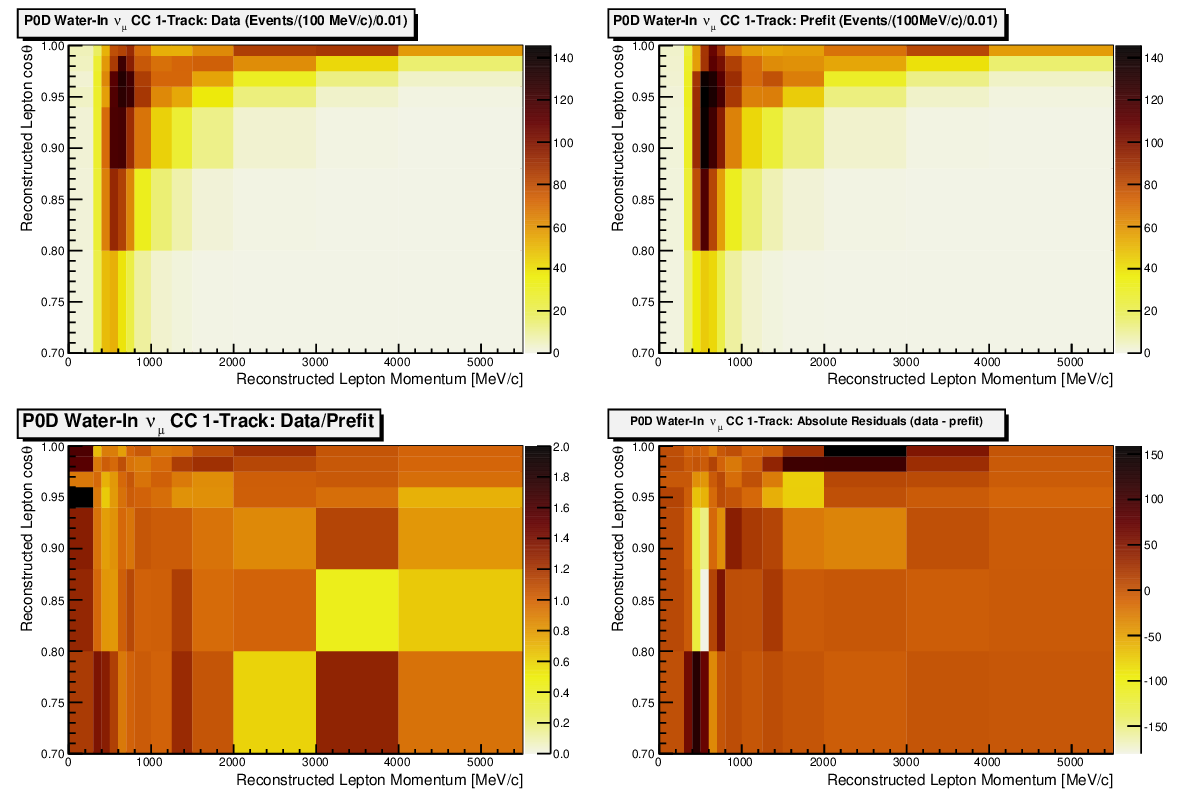
\includegraphics[width=0.99\textwidth]{Chapters/Figures/FitterResults/Prefit/output-0}
\par\end{centering}
}
\par\end{centering}
\caption[Prefit for the Water-In \numutitle{} in FHC Mode CC 1-Track Sample]{Data and prefit expectation for the $\pod$ Water-In $\protect\numu$
in FHC Mode CC 1-Track sample. Sub-figure (a) shows the momentum one-dimensional
profile in all but the highest momentum fit bin. Sub-figure (b) shows
the $\cos\theta$ one-dimensional profile in all but the highest angle
fit bin. Shown in both (a) and (b) is the ratio between data and the
prefit value. Sub-figure (c) shows a grid of two-dimensional data
and prefit distributions in the same phase space as (a) and (b). Moving
from top-left to bottom-right in (c) is the data, prefit, data to
prefit ratio, and data to prefit difference. \label{fig:Data-and-prefit-wtr-numu1Trk}
}
\end{figure}

\begin{figure}
\begin{centering}
\subfloat[Momentum in MeV/c]{\begin{centering}
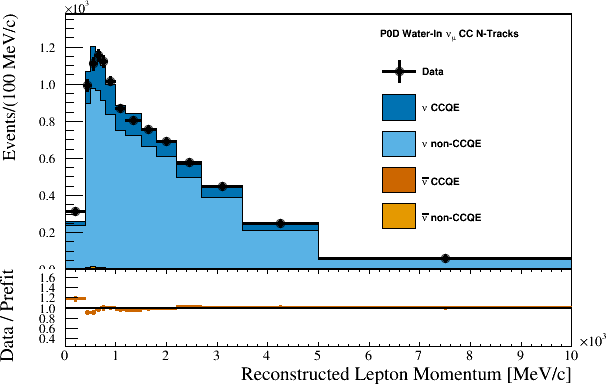
\includegraphics[width=0.48\textwidth]{Chapters/Figures/FitterResults/Prefit/png/P0D_Water_NuMu_CCNTracks_mumom_rxn_prefit}
\par\end{centering}
}\subfloat[$\cos\theta$]{\begin{centering}
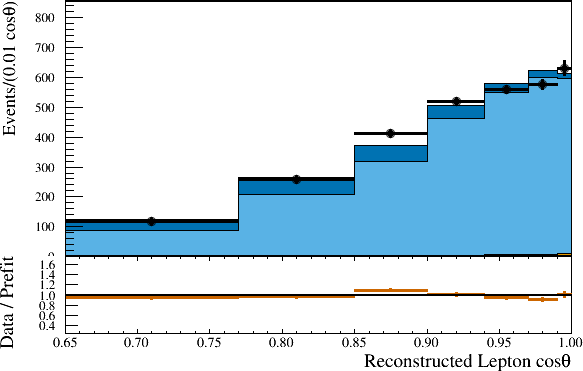
\includegraphics[width=0.48\textwidth]{Chapters/Figures/FitterResults/Prefit/png/P0D_Water_NuMu_CCNTracks_mucostheta_rxn_prefit}
\par\end{centering}
}
\par\end{centering}
\begin{centering}
\subfloat[Momentum-$\cos\theta$]{\begin{centering}
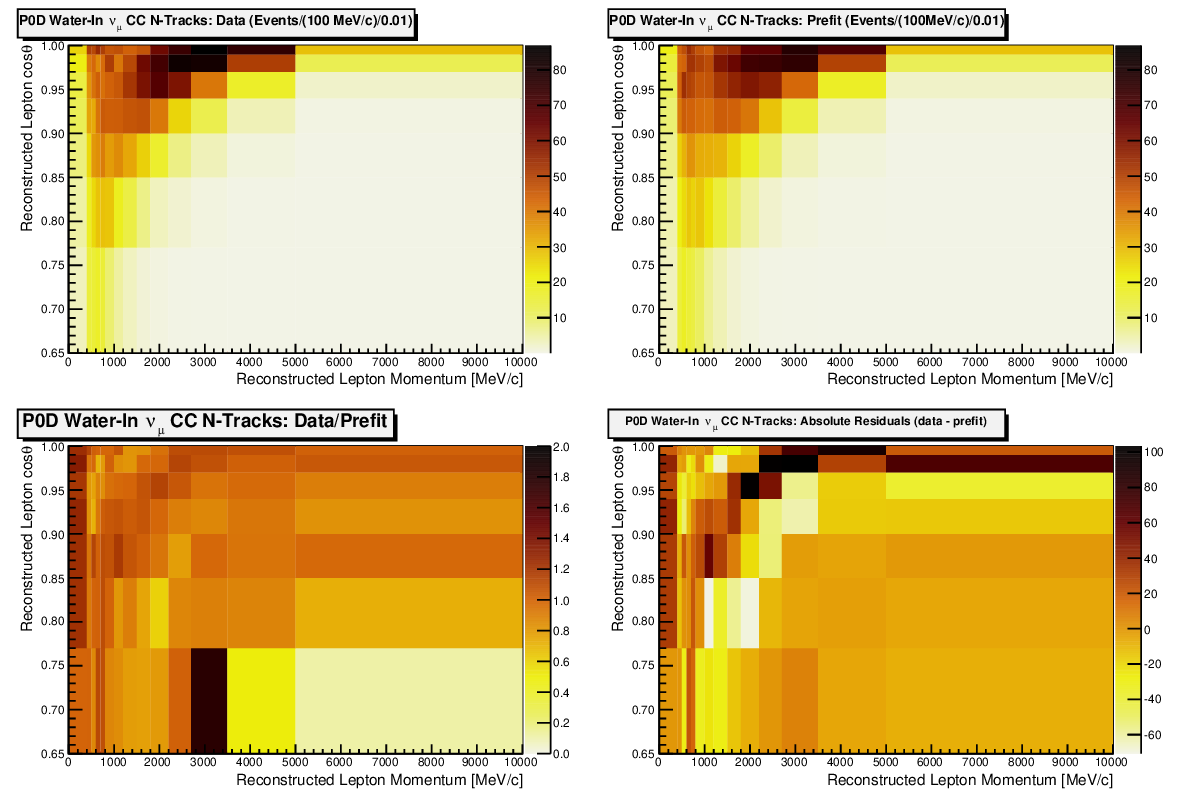
\includegraphics[width=0.99\textwidth]{Chapters/Figures/FitterResults/Prefit/output-1}
\par\end{centering}
}
\par\end{centering}
\caption[Prefit for the Water-In \numutitle{} in FHC Mode CC N-Tracks Sample]{Data and prefit expectation for the $\pod$ Water-In $\protect\numu$
in FHC Mode CC N-Tracks sample. Sub-figure (a) shows the momentum
one-dimensional profile in all but the highest momentum fit bin. Sub-figure
(b) shows the $\cos\theta$ one-dimensional profile in all but the
highest angle fit bin. Shown in both (a) and (b) is the ratio between
data and the prefit value. Sub-figure (c) shows a grid of two-dimensional
data and prefit distributions in the same phase space as (a) and (b).
Moving from top-left to bottom-right in (c) is the data, prefit, data
to prefit ratio, and data to prefit difference.\label{fig:Data-and-prefit-wtr-numuNTrks}
}
\end{figure}

\begin{figure}
\begin{centering}
\subfloat[Momentum in MeV/c]{\begin{centering}
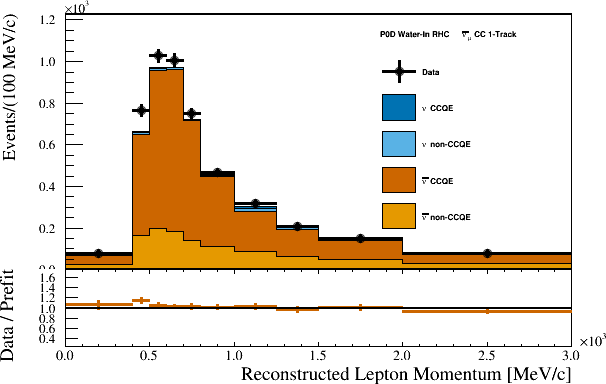
\includegraphics[width=0.48\textwidth]{Chapters/Figures/FitterResults/Prefit/png/P0D_Water_NuMubar_in_Anti_NuMode_CC1Track_mumom_rxn_prefit}
\par\end{centering}
}\subfloat[$\cos\theta$]{\begin{centering}
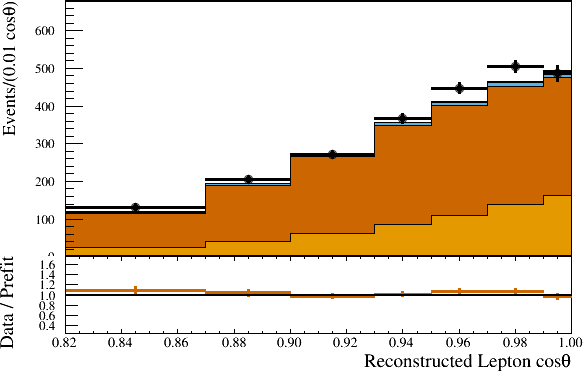
\includegraphics[width=0.48\textwidth]{Chapters/Figures/FitterResults/Prefit/png/P0D_Water_NuMubar_in_Anti_NuMode_CC1Track_mucostheta_rxn_prefit}
\par\end{centering}
}
\par\end{centering}
\begin{centering}
\subfloat[Momentum-$\cos\theta$]{\begin{centering}
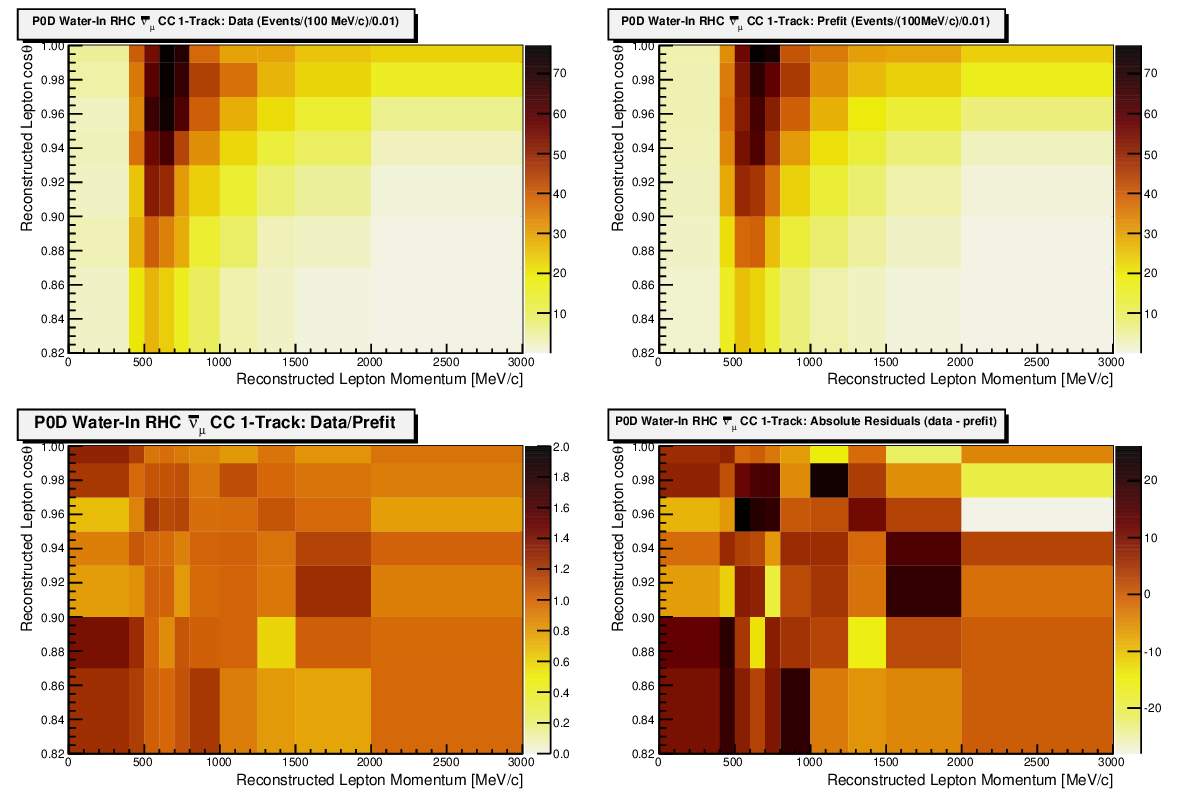
\includegraphics[width=0.99\textwidth]{Chapters/Figures/FitterResults/Prefit/output-2}
\par\end{centering}
}
\par\end{centering}
\caption[Prefit for the Water-In \numubartitle{} in RHC Mode CC 1-Track Sample]{Data and prefit expectation for the $\pod$ Water-In $\protect\numubar$
in RHC Mode CC 1-Track sample. Sub-figure (a) shows the momentum one-dimensional
profile in all but the highest momentum fit bin. Sub-figure (b) shows
the $\cos\theta$ one-dimensional profile in all but the highest angle
fit bin. Shown in both (a) and (b) is the ratio between data and the
prefit value. Sub-figure (c) shows a grid of two-dimensional data
and prefit distributions in the same phase space as (a) and (b). Moving
from top-left to bottom-right in (c) is the data, prefit, data to
prefit ratio, and data to prefit difference.\label{fig:Data-and-prefit-wtr-numubarRHC1Trk}
}
\end{figure}

\begin{figure}
\begin{centering}
\subfloat[Momentum in MeV/c]{\begin{centering}
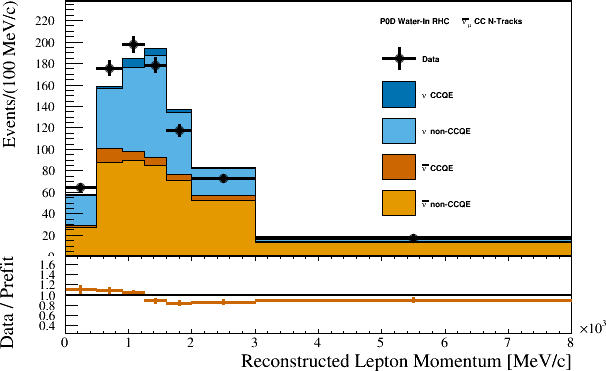
\includegraphics[width=0.48\textwidth]{Chapters/Figures/FitterResults/Prefit/png/P0D_Water_NuMubar_in_Anti_NuMode_CCNTracks_mumom_rxn_prefit}
\par\end{centering}
}\subfloat[$\cos\theta$]{\begin{centering}
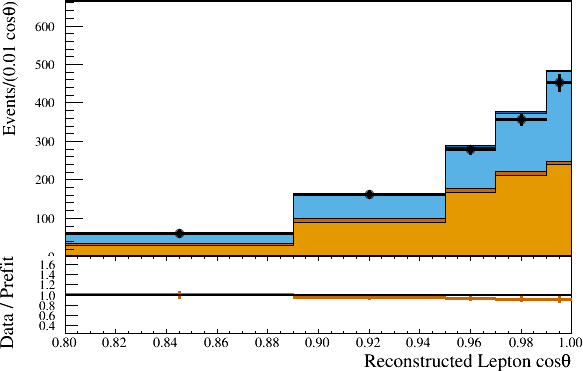
\includegraphics[width=0.48\textwidth]{Chapters/Figures/FitterResults/Prefit/png/P0D_Water_NuMubar_in_Anti_NuMode_CCNTracks_mucostheta_rxn_prefit}
\par\end{centering}
}
\par\end{centering}
\begin{centering}
\subfloat[Momentum-$\cos\theta$]{\begin{centering}
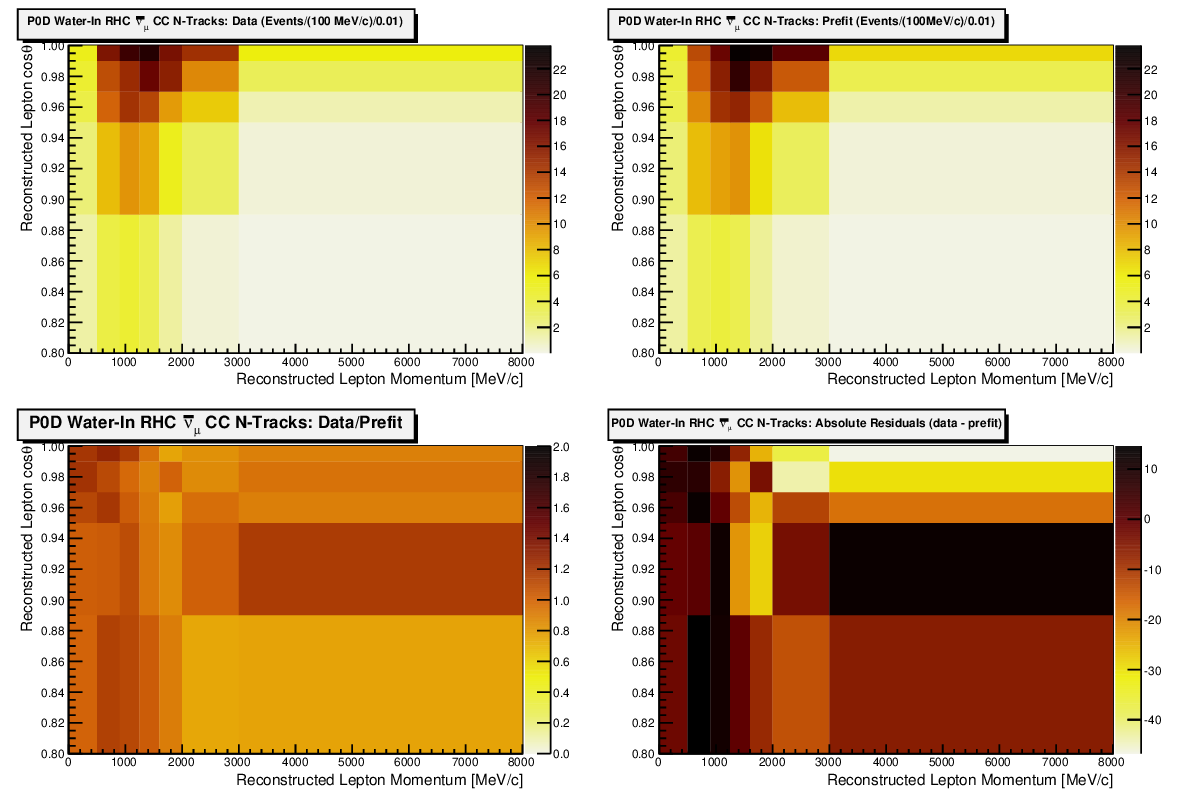
\includegraphics[width=0.99\textwidth]{Chapters/Figures/FitterResults/Prefit/output-3}
\par\end{centering}
}
\par\end{centering}
\caption[Prefit for the Water-In \numubartitle{} in RHC Mode CC N-Tracks Sample]{Data and prefit expectation for the $\pod$ Water-In $\protect\numubar$
in RHC Mode CC N-Tracks sample. Sub-figure (a) shows the momentum
one-dimensional profile in all but the highest momentum fit bin. Sub-figure
(b) shows the $\cos\theta$ one-dimensional profile in all but the
highest angle fit bin. Shown in both (a) and (b) is the ratio between
data and the prefit value. Sub-figure (c) shows a grid of two-dimensional
data and prefit distributions in the same phase space as (a) and (b).
Moving from top-left to bottom-right in (c) is the data, prefit, data
to prefit ratio, and data to prefit difference.\label{fig:Data-and-prefit-wtr-numubarRHCNTrks}
}
\end{figure}

\begin{figure}
\begin{centering}
\subfloat[Momentum in MeV/c]{\begin{centering}
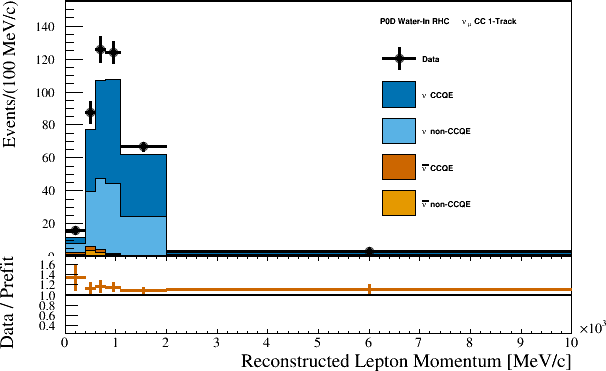
\includegraphics[width=0.48\textwidth]{Chapters/Figures/FitterResults/Prefit/png/P0D_Water_NuMu_Bkg_in_Anti_NuMode_CC1Track_mumom_rxn_prefit}
\par\end{centering}
}\subfloat[$\cos\theta$]{\begin{centering}
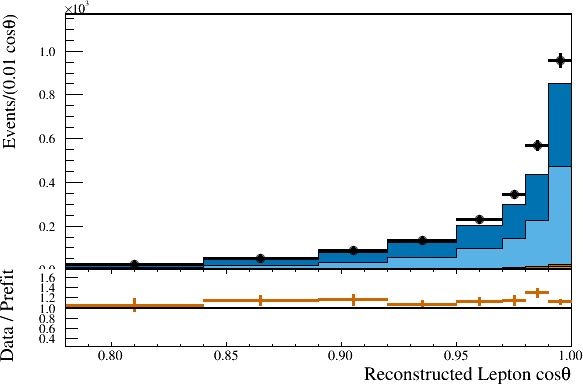
\includegraphics[width=0.48\textwidth]{Chapters/Figures/FitterResults/Prefit/png/P0D_Water_NuMu_Bkg_in_Anti_NuMode_CC1Track_mucostheta_rxn_prefit}
\par\end{centering}
}
\par\end{centering}
\begin{centering}
\subfloat[Momentum-$\cos\theta$]{\begin{centering}
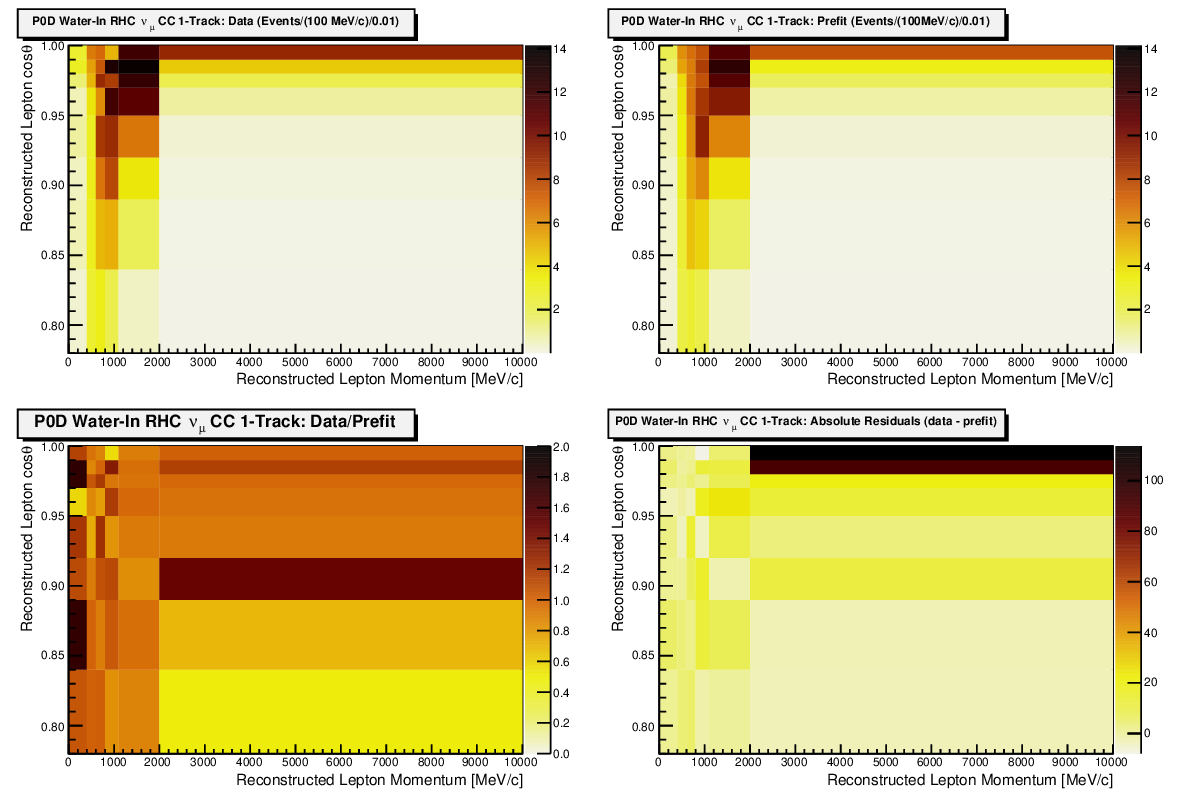
\includegraphics[width=0.99\textwidth]{Chapters/Figures/FitterResults/Prefit/output-4}
\par\end{centering}
}
\par\end{centering}
\caption[Prefit for the Water-In \numutitle{} in RHC Mode CC 1-Track Sample]{Data and prefit expectation for the $\pod$ Water-In $\protect\numu$
in RHC Mode CC 1-Track sample. Sub-figure (a) shows the momentum one-dimensional
profile in all but the highest momentum fit bin. Sub-figure (b) shows
the $\cos\theta$ one-dimensional profile in all but the highest angle
fit bin. Shown in both (a) and (b) is the ratio between data and the
prefit value. Sub-figure (c) shows a grid of two-dimensional data
and prefit distributions in the same phase space as (a) and (b). Moving
from top-left to bottom-right in (c) is the data, prefit, data to
prefit ratio, and data to prefit difference.\label{fig:Data-and-prefit-wtr-numuRHC1Trk}
}
\end{figure}

\begin{figure}
\begin{centering}
\subfloat[Momentum in MeV/c]{\begin{centering}
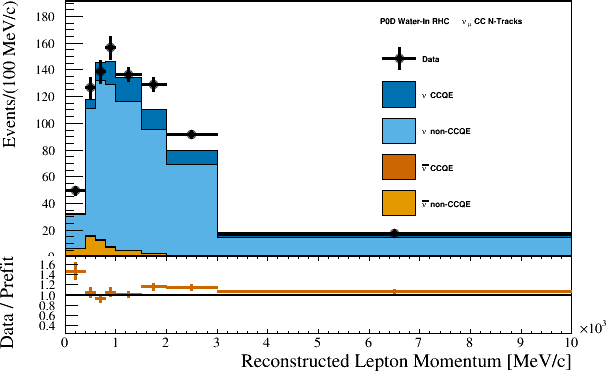
\includegraphics[width=0.48\textwidth]{Chapters/Figures/FitterResults/Prefit/png/P0D_Water_NuMu_Bkg_in_Anti_NuMode_CCNTracks_mumom_rxn_prefit}
\par\end{centering}
}\subfloat[$\cos\theta$]{\begin{centering}
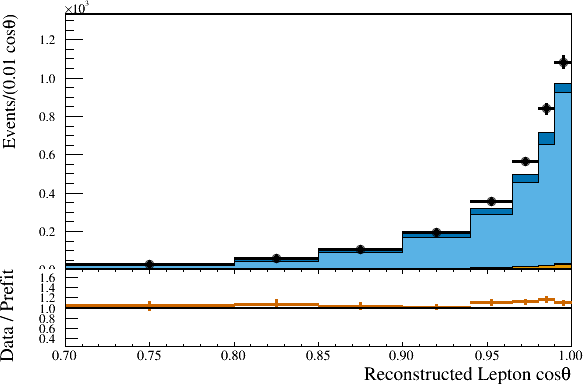
\includegraphics[width=0.48\textwidth]{Chapters/Figures/FitterResults/Prefit/png/P0D_Water_NuMu_Bkg_in_Anti_NuMode_CCNTracks_mucostheta_rxn_prefit}
\par\end{centering}
}
\par\end{centering}
\begin{centering}
\subfloat[Momentum-$\cos\theta$]{\begin{centering}
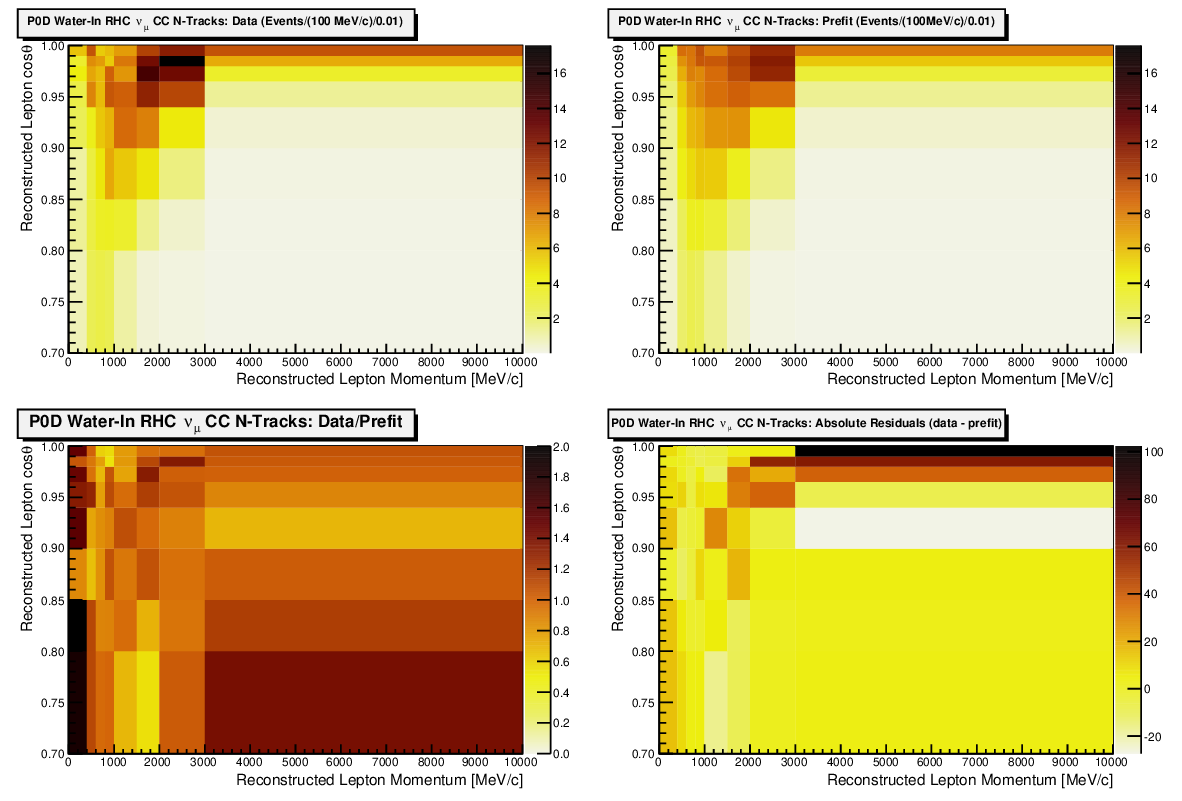
\includegraphics[width=0.99\textwidth]{Chapters/Figures/FitterResults/Prefit/output-5}
\par\end{centering}
}
\par\end{centering}
\caption[Prefit for the Water-In \numutitle{} in RHC Mode CC N-Tracks Sample]{Data and prefit expectation for the $\pod$ Water-In $\protect\numu$
in RHC Mode CC N-Tracks sample. Sub-figure (a) shows the momentum
one-dimensional profile in all but the highest momentum fit bin. Sub-figure
(b) shows the $\cos\theta$ one-dimensional profile in all but the
highest angle fit bin. Shown in both (a) and (b) is the ratio between
data and the prefit value. Sub-figure (c) shows a grid of two-dimensional
data and prefit distributions in the same phase space as (a) and (b).
Moving from top-left to bottom-right in (c) is the data, prefit, data
to prefit ratio, and data to prefit difference.\label{fig:Data-and-prefit-wtr-numuRHCNTrks}
}
\end{figure}

\begin{figure}
\begin{centering}
\subfloat[Momentum in MeV/c]{\begin{centering}
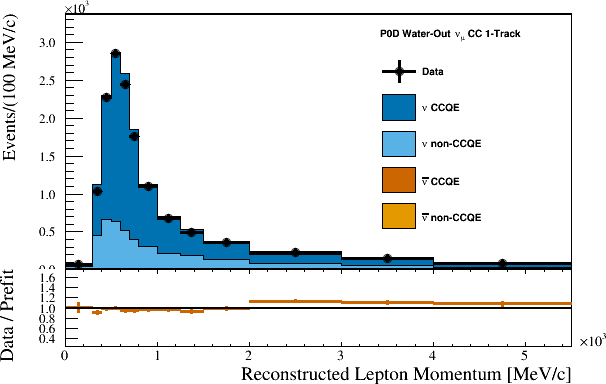
\includegraphics[width=0.48\textwidth]{Chapters/Figures/FitterResults/Prefit/png/P0D_Air_NuMu_CC1Track_mumom_rxn_prefit}
\par\end{centering}
}\subfloat[$\cos\theta$]{\begin{centering}
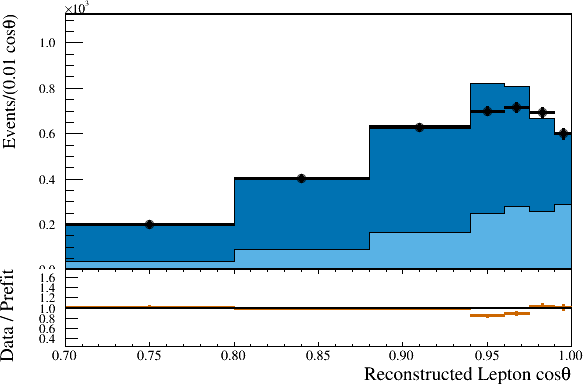
\includegraphics[width=0.48\textwidth]{Chapters/Figures/FitterResults/Prefit/png/P0D_Air_NuMu_CC1Track_mucostheta_rxn_prefit}
\par\end{centering}
}
\par\end{centering}
\begin{centering}
\subfloat[Momentum-$\cos\theta$]{\begin{centering}
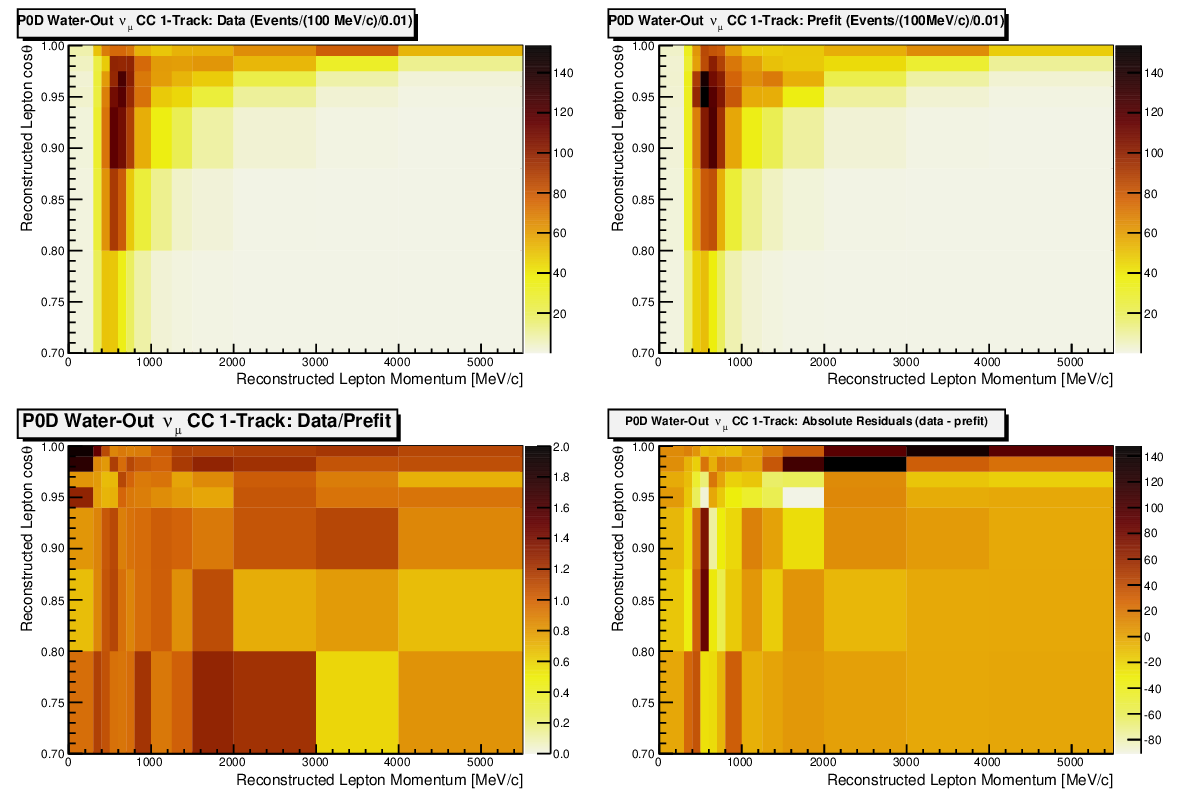
\includegraphics[width=0.99\textwidth]{Chapters/Figures/FitterResults/Prefit/output-6}
\par\end{centering}
}
\par\end{centering}
\caption[Prefit for the Water-Out \numutitle{} in FHC Mode CC 1-Track Sample]{Data and prefit expectation for the $\pod$ Water-Out $\protect\numu$
in FHC Mode CC 1-Track sample. Sub-figure (a) shows the momentum one-dimensional
profile in all but the highest momentum fit bin. Sub-figure (b) shows
the $\cos\theta$ one-dimensional profile in all but the highest angle
fit bin. Shown in both (a) and (b) is the ratio between data and the
prefit value. Sub-figure (c) shows a grid of two-dimensional data
and prefit distributions in the same phase space as (a) and (b). Moving
from top-left to bottom-right in (c) is the data, prefit, data to
prefit ratio, and data to prefit difference. \label{fig:Data-and-prefit-air-numu1Trk}
}
\end{figure}

\begin{figure}
\begin{centering}
\subfloat[Momentum in MeV/c]{\begin{centering}
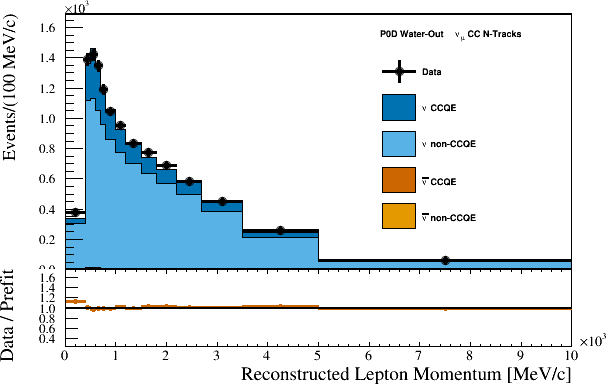
\includegraphics[width=0.48\textwidth]{Chapters/Figures/FitterResults/Prefit/png/P0D_Air_NuMu_CCNTracks_mumom_rxn_prefit}
\par\end{centering}
}\subfloat[$\cos\theta$]{\begin{centering}
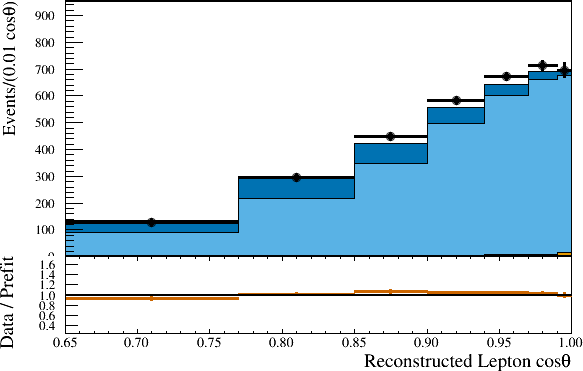
\includegraphics[width=0.48\textwidth]{Chapters/Figures/FitterResults/Prefit/png/P0D_Air_NuMu_CCNTracks_mucostheta_rxn_prefit}
\par\end{centering}
}
\par\end{centering}
\begin{centering}
\subfloat[Momentum-$\cos\theta$]{\begin{centering}
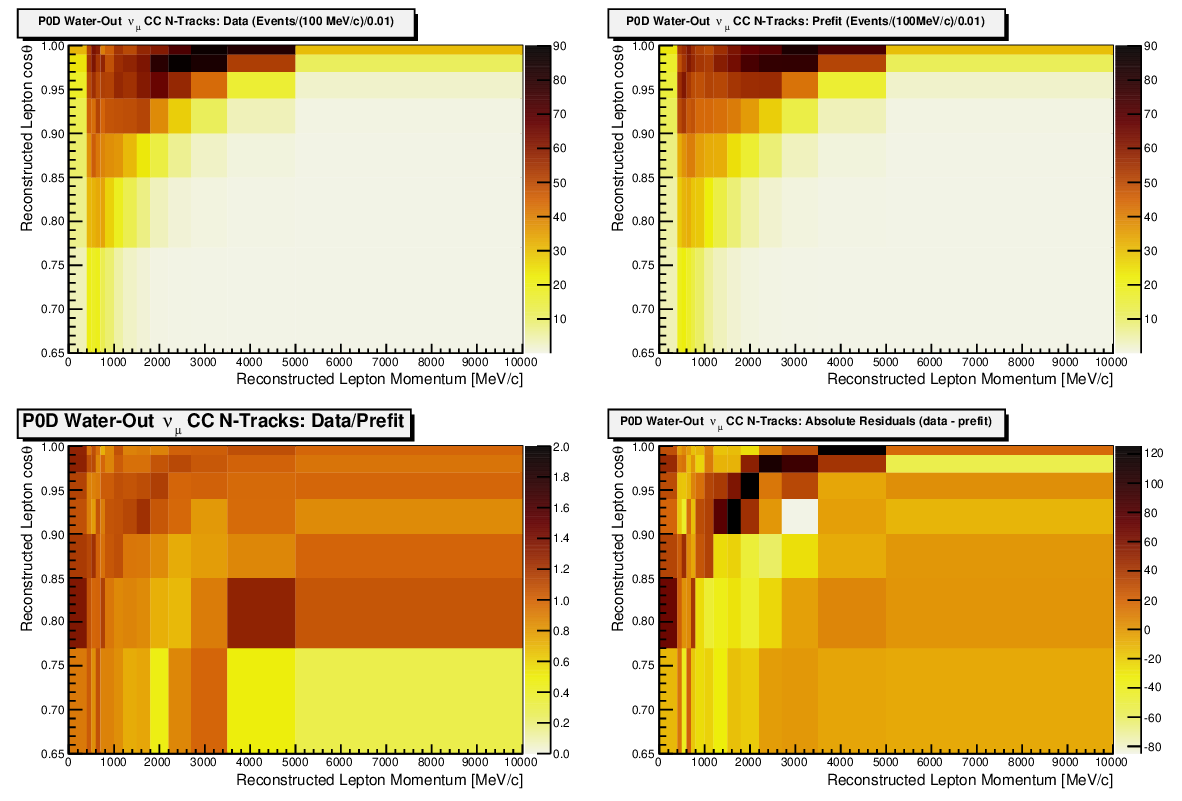
\includegraphics[width=0.99\textwidth]{Chapters/Figures/FitterResults/Prefit/output-7}
\par\end{centering}
}
\par\end{centering}
\caption[Prefit for the Water-Out \numutitle{} in FHC Mode CC N-Tracks Sample]{Data and prefit expectation for the $\pod$ Water-Out $\protect\numu$
in FHC Mode CC N-Tracks sample. Sub-figure (a) shows the momentum
one-dimensional profile in all but the highest momentum fit bin. Sub-figure
(b) shows the $\cos\theta$ one-dimensional profile in all but the
highest angle fit bin. Shown in both (a) and (b) is the ratio between
data and the prefit value. Sub-figure (c) shows a grid of two-dimensional
data and prefit distributions in the same phase space as (a) and (b).
Moving from top-left to bottom-right in (c) is the data, prefit, data
to prefit ratio, and data to prefit difference. \label{fig:Data-and-prefit-air-numuNTrks}
}
\end{figure}

\begin{figure}
\begin{centering}
\subfloat[Momentum in MeV/c]{\begin{centering}
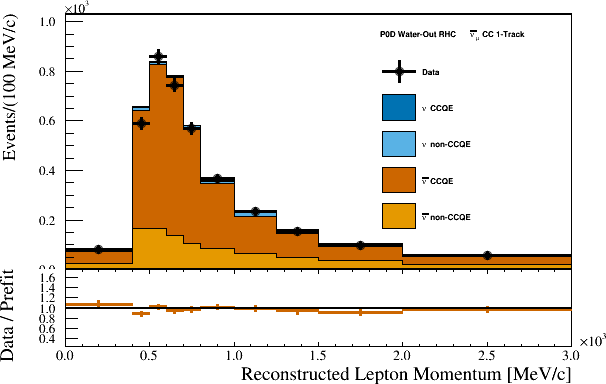
\includegraphics[width=0.48\textwidth]{Chapters/Figures/FitterResults/Prefit/png/P0D_Air_NuMubar_in_Anti_NuMode_CC1Track_mumom_rxn_prefit}
\par\end{centering}
}\subfloat[$\cos\theta$]{\begin{centering}
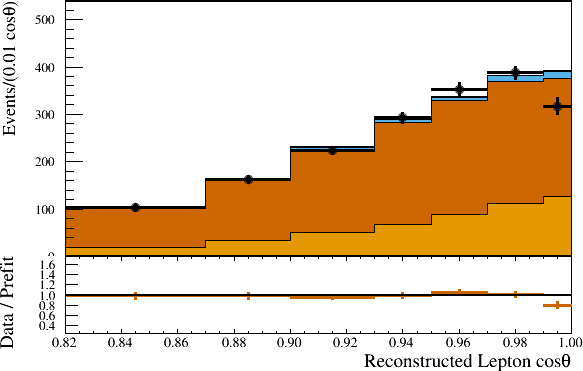
\includegraphics[width=0.48\textwidth]{Chapters/Figures/FitterResults/Prefit/png/P0D_Air_NuMubar_in_Anti_NuMode_CC1Track_mucostheta_rxn_prefit}
\par\end{centering}
}
\par\end{centering}
\begin{centering}
\subfloat[Momentum-$\cos\theta$]{\begin{centering}
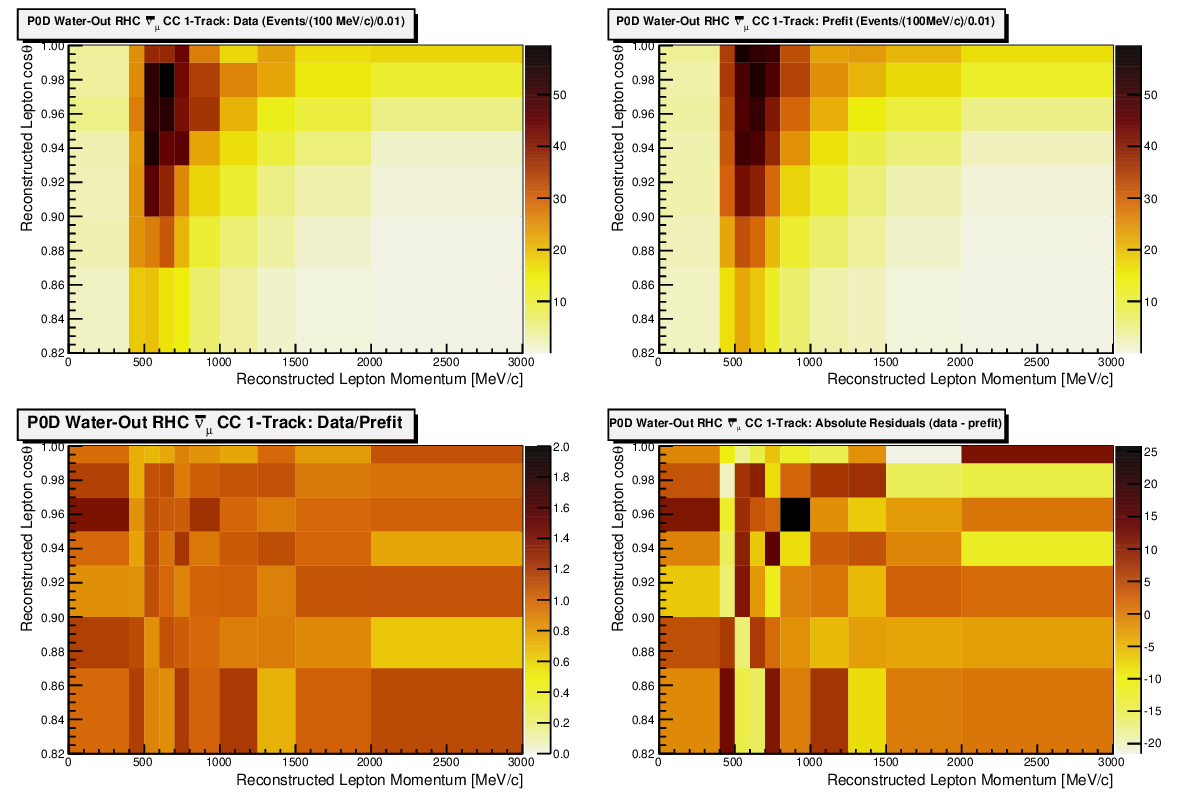
\includegraphics[width=0.99\textwidth]{Chapters/Figures/FitterResults/Prefit/output-8}
\par\end{centering}
}
\par\end{centering}
\caption[Prefit for the Water-Out \numubartitle{} in RHC Mode CC 1-Track Sample]{Data and prefit expectation for the $\pod$ Water-Out $\protect\numubar$
in RHC Mode CC 1-Track sample. Sub-figure (a) shows the momentum one-dimensional
profile in all but the highest momentum fit bin. Sub-figure (b) shows
the $\cos\theta$ one-dimensional profile in all but the highest angle
fit bin. Shown in both (a) and (b) is the ratio between data and the
prefit value. Sub-figure (c) shows a grid of two-dimensional data
and prefit distributions in the same phase space as (a) and (b). Moving
from top-left to bottom-right in (c) is the data, prefit, data to
prefit ratio, and data to prefit difference. \label{fig:Data-and-prefit-air-numubarRHC1Trk}
}
\end{figure}

\begin{figure}
\begin{centering}
\subfloat[Momentum in MeV/c]{\begin{centering}
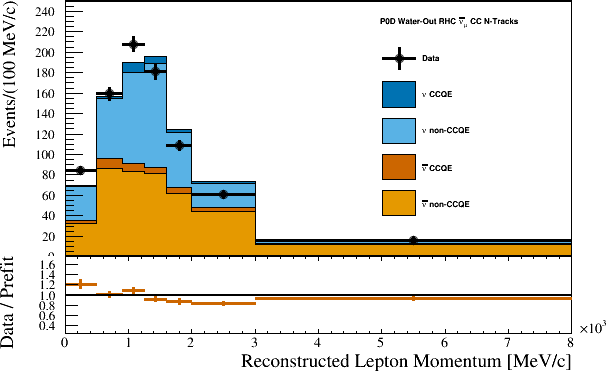
\includegraphics[width=0.48\textwidth]{Chapters/Figures/FitterResults/Prefit/png/P0D_Air_NuMubar_in_Anti_NuMode_CCNTracks_mumom_rxn_prefit}
\par\end{centering}
}\subfloat[$\cos\theta$]{\begin{centering}
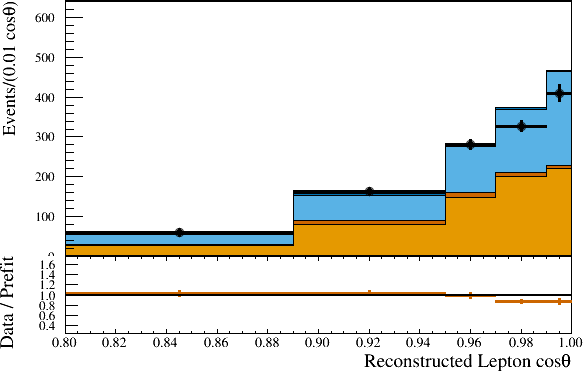
\includegraphics[width=0.48\textwidth]{Chapters/Figures/FitterResults/Prefit/png/P0D_Air_NuMubar_in_Anti_NuMode_CCNTracks_mucostheta_rxn_prefit}
\par\end{centering}
}
\par\end{centering}
\begin{centering}
\subfloat[Momentum-$\cos\theta$]{\begin{centering}
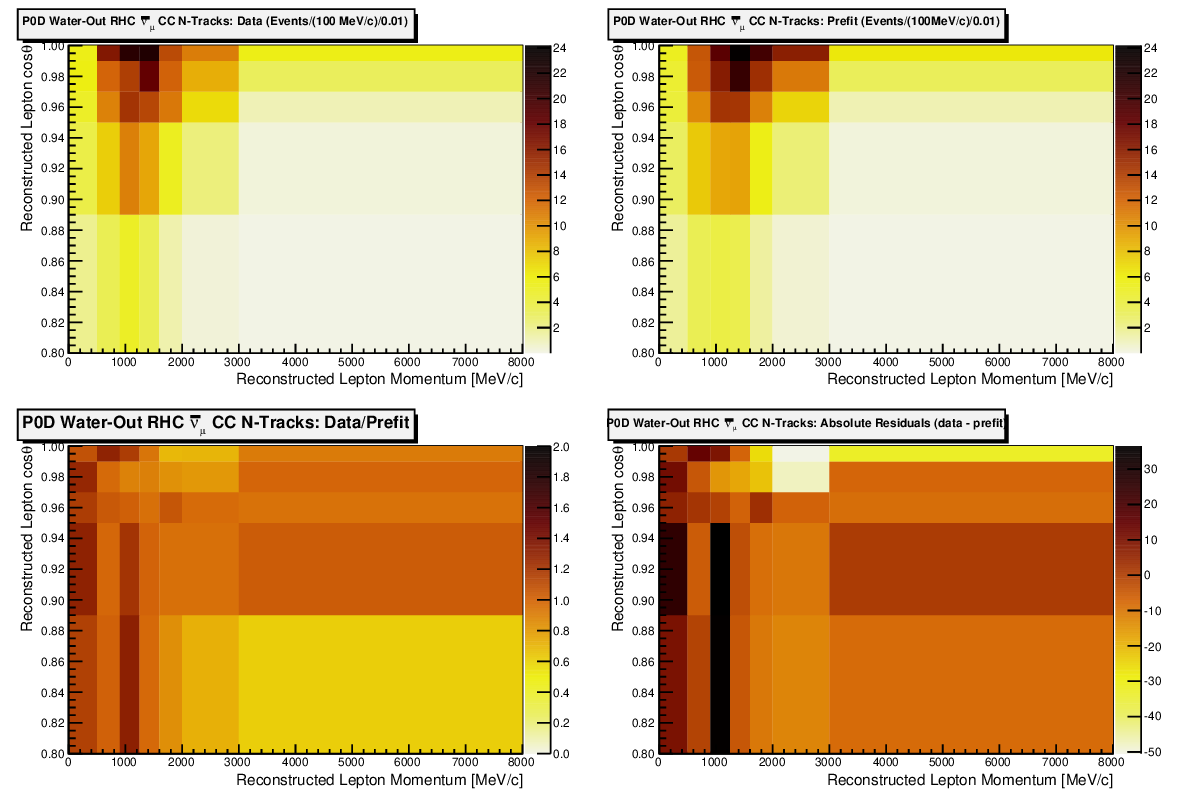
\includegraphics[width=0.99\textwidth]{Chapters/Figures/FitterResults/Prefit/output-9}
\par\end{centering}
}
\par\end{centering}
\caption[Prefit for the Water-Out \numubartitle{} in RHC Mode CC N-Tracks
Sample]{Data and prefit expectation for the $\pod$ Water-Out $\protect\numubar$
in RHC Mode CC N-Tracks sample. Sub-figure (a) shows the momentum
one-dimensional profile in all but the highest momentum fit bin. Sub-figure
(b) shows the $\cos\theta$ one-dimensional profile in all but the
highest angle fit bin. Shown in both (a) and (b) is the ratio between
data and the prefit value. Sub-figure (c) shows a grid of two-dimensional
data and prefit distributions in the same phase space as (a) and (b).
Moving from top-left to bottom-right in (c) is the data, prefit, data
to prefit ratio, and data to prefit difference. \label{fig:Data-and-prefit-air-numubarRHCNTrks}
}
\end{figure}

\begin{figure}
\begin{centering}
\subfloat[Momentum in MeV/c]{\begin{centering}
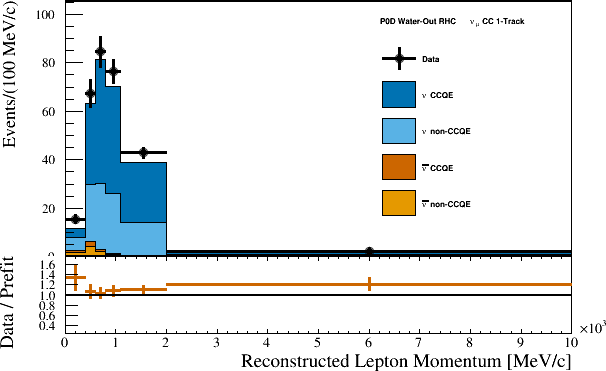
\includegraphics[width=0.48\textwidth]{Chapters/Figures/FitterResults/Prefit/png/P0D_Air_NuMu_Bkg_in_Anti_NuMode_CC1Track_mumom_rxn_prefit}
\par\end{centering}
}\subfloat[$\cos\theta$]{\begin{centering}
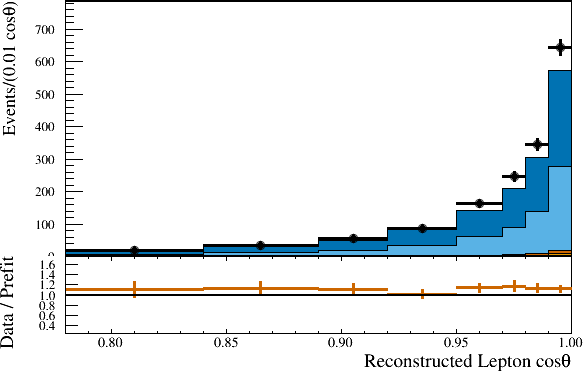
\includegraphics[width=0.48\textwidth]{Chapters/Figures/FitterResults/Prefit/png/P0D_Air_NuMu_Bkg_in_Anti_NuMode_CC1Track_mucostheta_rxn_prefit}
\par\end{centering}
}
\par\end{centering}
\begin{centering}
\subfloat[Momentum-$\cos\theta$]{\begin{centering}
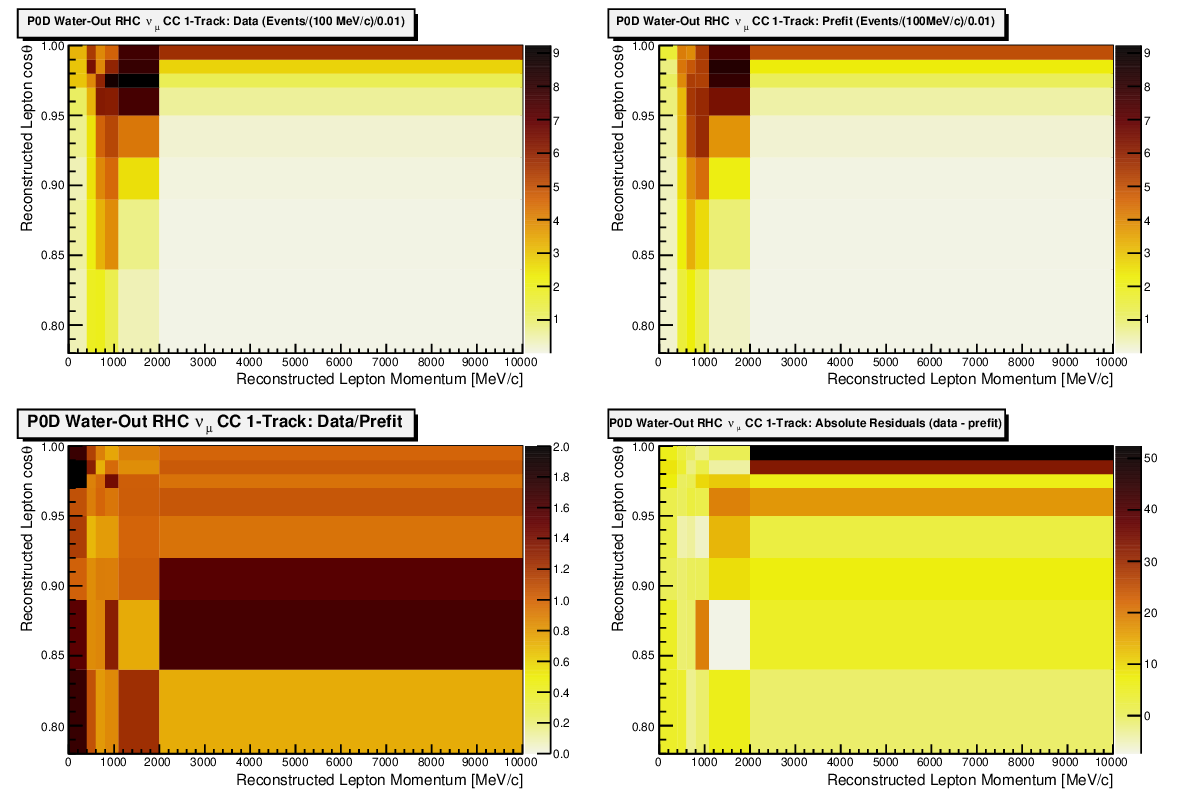
\includegraphics[width=0.99\textwidth]{Chapters/Figures/FitterResults/Prefit/output-10}
\par\end{centering}
}
\par\end{centering}
\caption[Prefit for the Water-Out \numutitle{} in RHC Mode CC 1-Track Sample]{Data and prefit expectation for the $\pod$ Water-Out $\protect\numu$
in RHC Mode CC 1-Track sample. Sub-figure (a) shows the momentum one-dimensional
profile in all but the highest momentum fit bin. Sub-figure (b) shows
the $\cos\theta$ one-dimensional profile in all but the highest angle
fit bin. Shown in both (a) and (b) is the ratio between data and the
prefit value. Sub-figure (c) shows a grid of two-dimensional data
and prefit distributions in the same phase space as (a) and (b). Moving
from top-left to bottom-right in (c) is the data, prefit, data to
prefit ratio, and data to prefit difference. \label{fig:Data-and-prefit-air-numuRHC1Trk}
}
\end{figure}

\begin{figure}
\begin{centering}
\subfloat[Momentum in MeV/c]{\begin{centering}
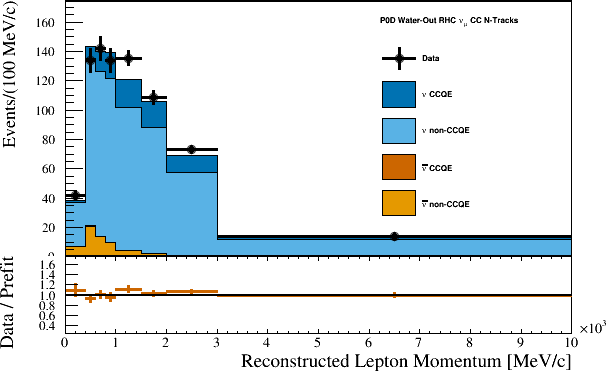
\includegraphics[width=0.48\textwidth]{Chapters/Figures/FitterResults/Prefit/png/P0D_Air_NuMu_Bkg_in_Anti_NuMode_CCNTracks_mumom_rxn_prefit}
\par\end{centering}
}\subfloat[$\cos\theta$]{\begin{centering}
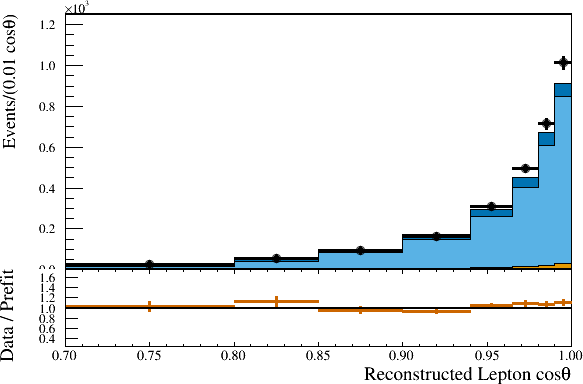
\includegraphics[width=0.48\textwidth]{Chapters/Figures/FitterResults/Prefit/png/P0D_Air_NuMu_Bkg_in_Anti_NuMode_CCNTracks_mucostheta_rxn_prefit}
\par\end{centering}
}
\par\end{centering}
\begin{centering}
\subfloat[Momentum-$\cos\theta$]{\begin{centering}
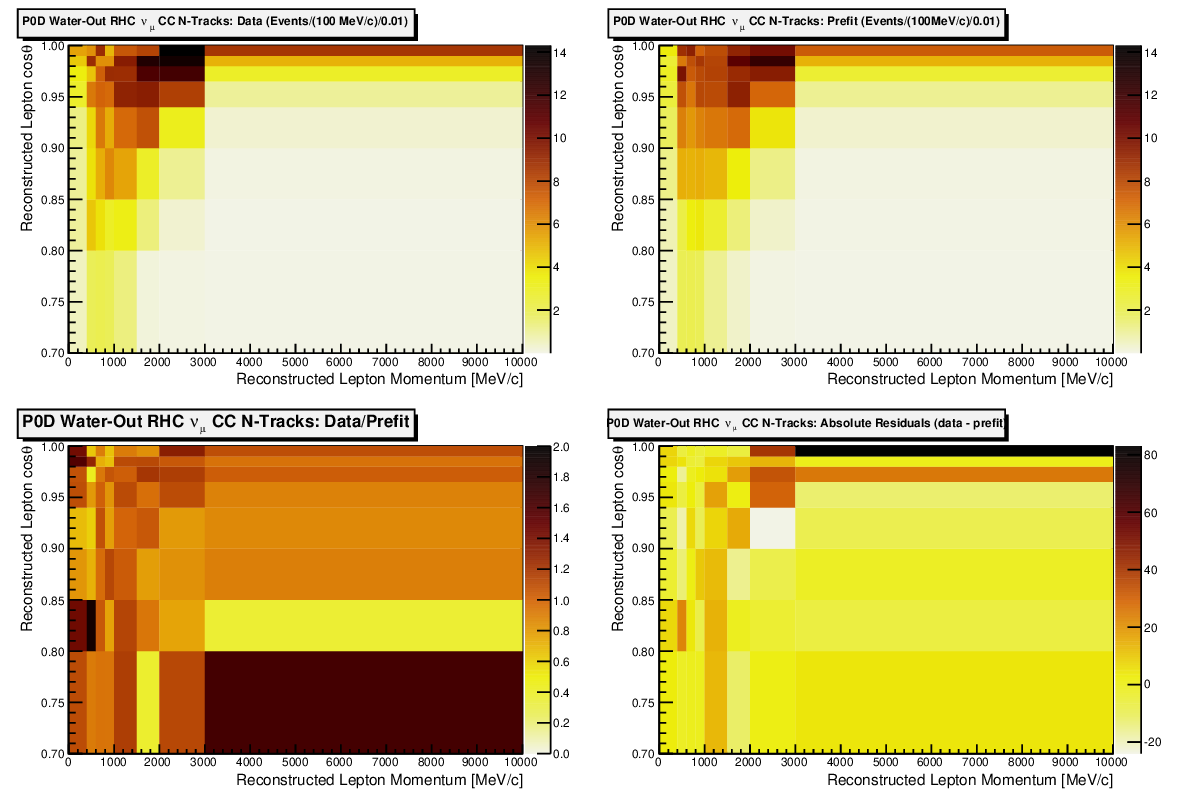
\includegraphics[width=0.99\textwidth]{Chapters/Figures/FitterResults/Prefit/output-11}
\par\end{centering}
}
\par\end{centering}
\caption[Prefit for the Water-Out \numutitle{} in RHC Mode CC N-Tracks Sample]{Data and prefit expectation for the $\pod$ Water-Out $\protect\numu$
in RHC Mode CC N-Tracks sample. Sub-figure (a) shows the momentum
one-dimensional profile in all but the highest momentum fit bin. Sub-figure
(b) shows the $\cos\theta$ one-dimensional profile in all but the
highest angle fit bin. Shown in both (a) and (b) is the ratio between
data and the prefit value. Sub-figure (c) shows a grid of two-dimensional
data and prefit distributions in the same phase space as (a) and (b).
Moving from top-left to bottom-right in (c) is the data, prefit, data
to prefit ratio, and data to prefit difference. \label{fig:Data-and-prefit-air-numuRHCNTrks}
}
\end{figure}


\section{Postfit Results\label{sec:Postfit-Results}}

The results of the $\pod$-only BANFF fit are presented here. Starting
with an initial test statistic of $\chi_{\text{ND}280}^{2}=3022.2$,
the MINUIT optimization routine required 149661 iterations to find
the global minimum at $\hat{\chi}_{\text{ND}280}^{2}=1412.28$. An
additional 176000 iterations were required to calculate the Hessian
matrix. The computing resources used for the fit are presented in
Appendix \prettyref{chap:Computing-Resources}.

Specific topics on the postfit results are presented in the following
order. First is an examination of the postfit samples in one-dimensional
profiles and two-dimensional spaces. The second, final topic is a
comparison of the parameter values among the prefit, $\pod$-only,
and FGD-only results.

\subsection{Postfit Sample Distributions}

Presented below are the 12 samples again, but with the parameters
extracted from the fit applied to the fit bins. This ensures that
we have a) not altered the data, and b) that the fitted parameters
(postfit) have improved the data matching as a result. The samples
are shown in \prettyref{fig:Data-and-postfit-wtr-numu1Trk} to \prettyref{fig:Data-and-postfit-air-numuRHCNTrks}
in the same order as presented in the previous section.

We see an improved agreement between the postfit prediction and the
data. Still, there is some poor data matching, in particular, in the
lowest momentum bins. This seems to be balanced between the water-in
and water-out modes since the flux parameters affect the samples the
same way. Given there still is tension in those lowest momentum bins,
perhaps the water mass systematic uncertainty was under estimated
in this analysis.

It is hypothesized that if the mass systematic was indeed underestimated,
the data to postfit ratio would converge towards 1 with decreasing
$\cos\theta$ in the water-in sample's lowest momentum bins. If better
agreement is observed in those higher angle bins compared to the lower
angle bins, this would support the idea that the mass systematic uncertainty
is underestimated. However, there was a weak trend observed in the
water-in samples, and such a weak one could be coincidental given
the number of bins. Therefore, it is difficult to draw any conclusions
if the mass systematic uncertainty was underestimated until other
constraints are provided.

\begin{figure}
\begin{centering}
\subfloat[Momentum in MeV/c]{\begin{centering}
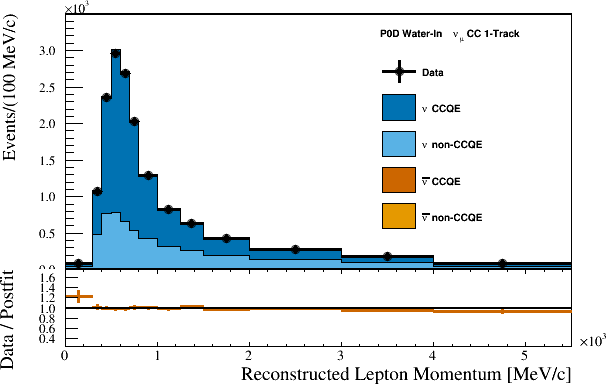
\includegraphics[width=0.48\textwidth]{Chapters/Figures/FitterResults/Postfit/png/P0D_Water_NuMu_CC1Track_mumom_rxn_postfit}
\par\end{centering}
}\subfloat[$\cos\theta$]{\begin{centering}
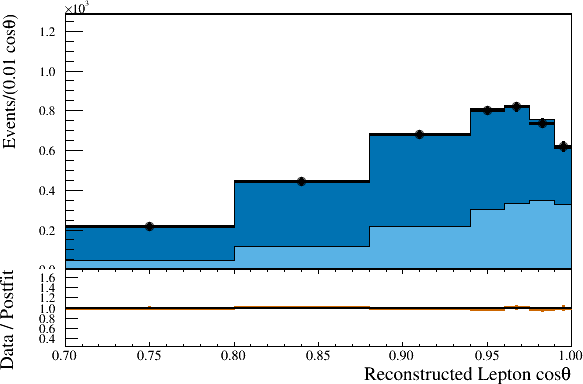
\includegraphics[width=0.48\textwidth]{Chapters/Figures/FitterResults/Postfit/png/P0D_Water_NuMu_CC1Track_mucostheta_rxn_postfit}
\par\end{centering}
}
\par\end{centering}
\begin{centering}
\subfloat[Momentum-$\cos\theta$]{\begin{centering}
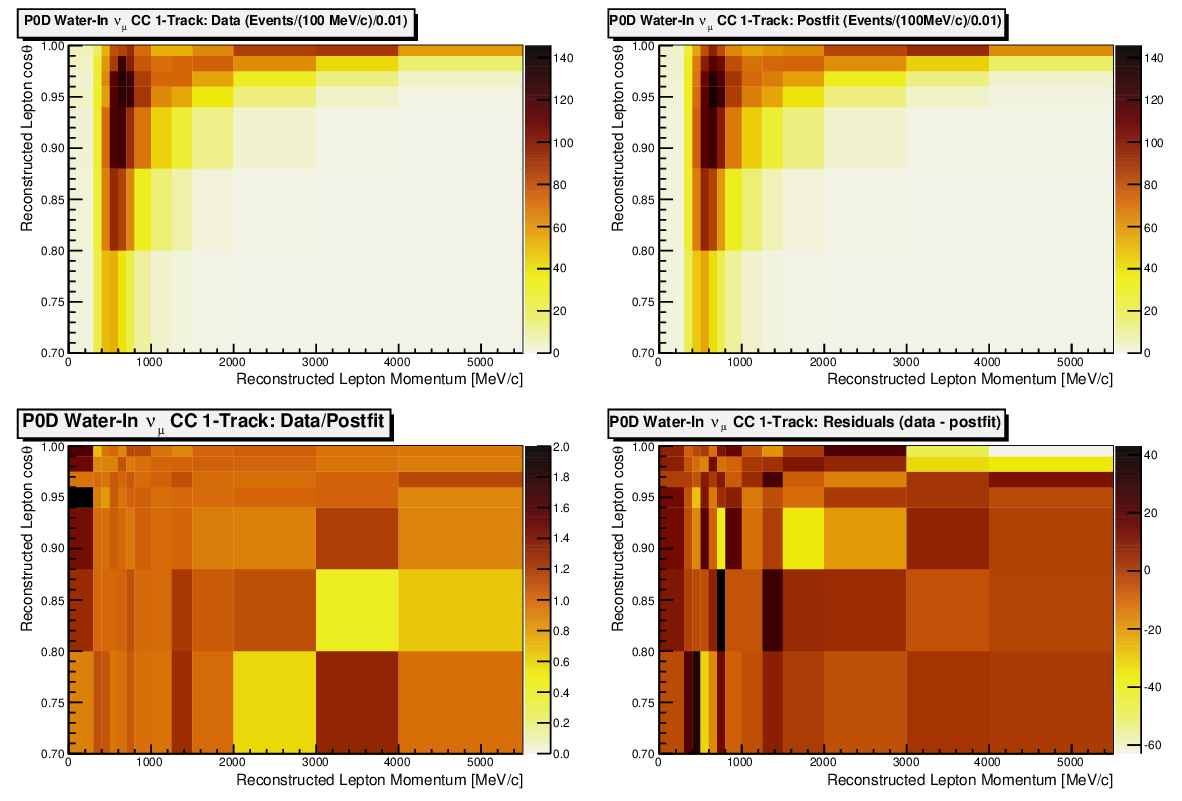
\includegraphics[width=0.99\textwidth]{Chapters/Figures/FitterResults/Postfit/output-0}
\par\end{centering}
}
\par\end{centering}
\caption[Postfit for the Water-In \numutitle{} in FHC Mode CC 1-Track Sample]{Data and postfit for the $\pod$ Water-In $\protect\numu$ in FHC
Mode CC 1-Track sample. Sub-figure (a) shows the momentum one-dimensional
profile in all but the highest momentum fit bin. Sub-figure (b) shows
the $\cos\theta$ one-dimensional profile in all but the highest angle
fit bin. Shown in both (a) and (b) is the ratio between data and the
postfit value. Sub-figure (c) shows a grid of two-dimensional data
and postfit distributions in the same phase space as (a) and (b).
Moving from top-left to bottom-right in (c) is the data, postfit,
data to postfit ratio, and data to postfit difference. \label{fig:Data-and-postfit-wtr-numu1Trk}
}
\end{figure}

\begin{figure}
\begin{centering}
\subfloat[Momentum in MeV/c]{\begin{centering}
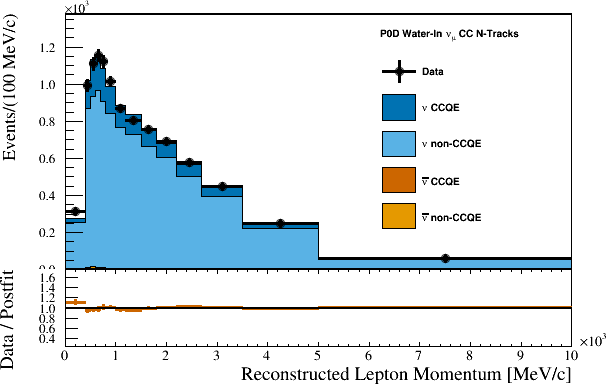
\includegraphics[width=0.48\textwidth]{Chapters/Figures/FitterResults/Postfit/png/P0D_Water_NuMu_CCNTracks_mumom_rxn_postfit}
\par\end{centering}
}\subfloat[$\cos\theta$]{\begin{centering}
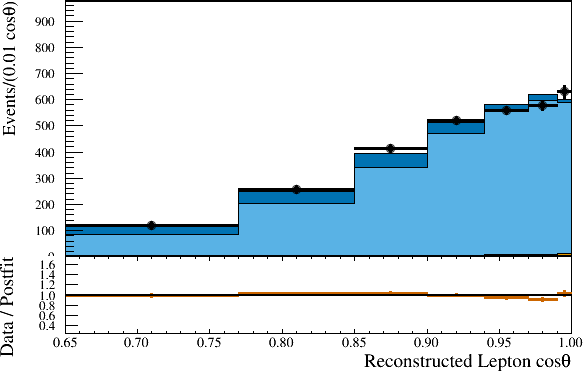
\includegraphics[width=0.48\textwidth]{Chapters/Figures/FitterResults/Postfit/png/P0D_Water_NuMu_CCNTracks_mucostheta_rxn_postfit}
\par\end{centering}
}
\par\end{centering}
\begin{centering}
\subfloat[Momentum-$\cos\theta$]{\begin{centering}
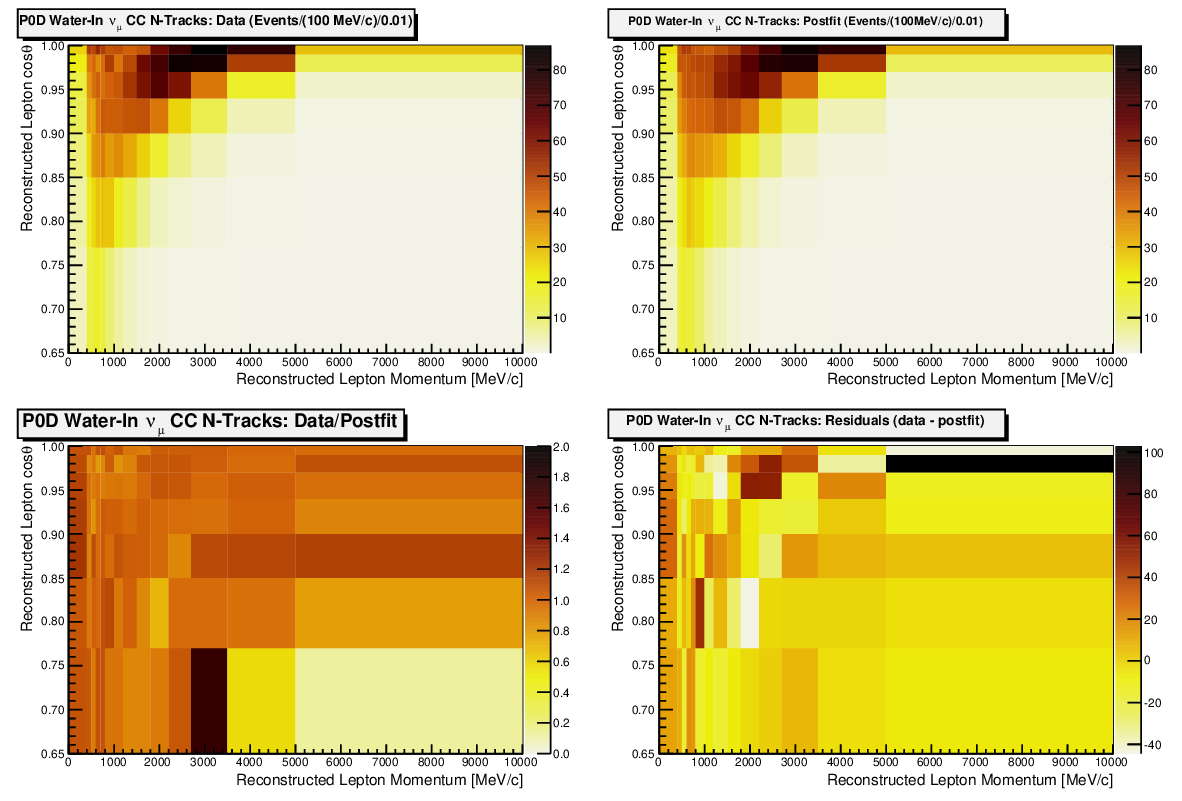
\includegraphics[width=0.99\textwidth]{Chapters/Figures/FitterResults/Postfit/output-1}
\par\end{centering}
}
\par\end{centering}
\caption[Postfit for the Water-In \numutitle{} in FHC Mode CC N-Tracks Sample]{Data and postfit for the $\pod$ Water-In $\protect\numu$ in FHC
Mode CC 1-Track sample. Sub-figure (a) shows the momentum one-dimensional
profile in all but the highest momentum fit bin. Sub-figure (b) shows
the $\cos\theta$ one-dimensional profile in all but the highest angle
fit bin. Shown in both (a) and (b) is the ratio between data and the
postfit value. Sub-figure (c) shows a grid of two-dimensional data
and postfit distributions in the same phase space as (a) and (b).
Moving from top-left to bottom-right in (c) is the data, postfit,
data to postfit ratio, and data to postfit difference. \label{fig:Data-and-postfit-wtr-numuNTrks}
}
\end{figure}

\begin{figure}
\begin{centering}
\subfloat[Momentum in MeV/c]{\begin{centering}
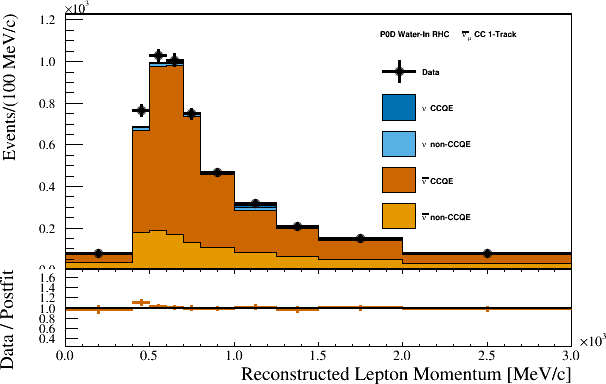
\includegraphics[width=0.45\textwidth,height=0.45\textheight,keepaspectratio]{Chapters/Figures/FitterResults/Postfit/png/P0D_Water_NuMubar_in_Anti_NuMode_CC1Track_mumom_rxn_postfit}
\par\end{centering}
}\subfloat[$\cos\theta$]{\begin{centering}
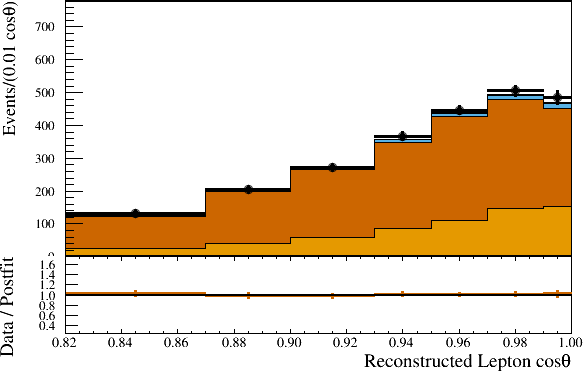
\includegraphics[width=0.45\textwidth,height=0.45\textheight,keepaspectratio]{Chapters/Figures/FitterResults/Postfit/png/P0D_Water_NuMubar_in_Anti_NuMode_CC1Track_mucostheta_rxn_postfit}
\par\end{centering}
}
\par\end{centering}
\begin{centering}
\subfloat[Momentum-$\cos\theta$]{\begin{centering}
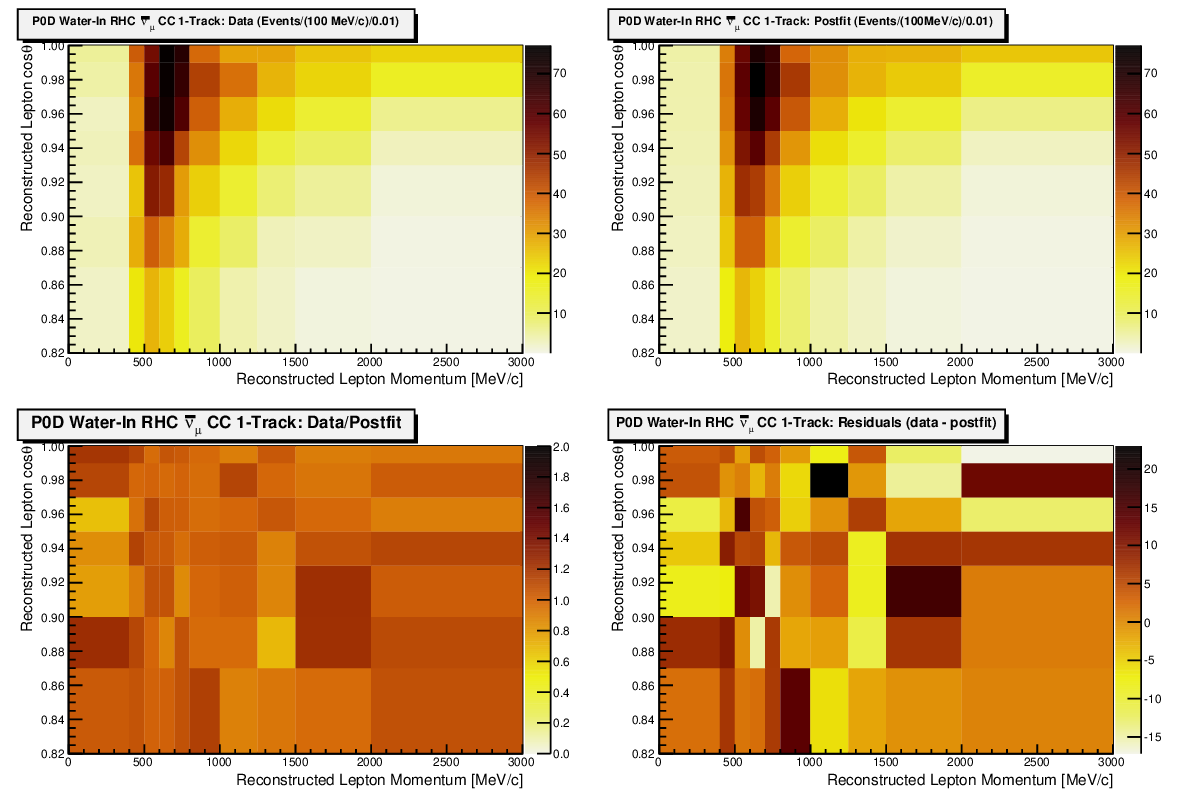
\includegraphics[width=0.99\textwidth]{Chapters/Figures/FitterResults/Postfit/output-2}
\par\end{centering}
}
\par\end{centering}
\caption[Postfit for the Water-In \numubartitle{} in RHC Mode CC 1-Track Sample]{Data and postfit for the $\pod$ Water-In $\protect\numubar$ in RHC
Mode CC 1-Track sample. Sub-figure (a) shows the momentum one-dimensional
profile in all but the highest momentum fit bin. Sub-figure (b) shows
the $\cos\theta$ one-dimensional profile in all but the highest angle
fit bin. Shown in both (a) and (b) is the ratio between data and the
postfit value. Sub-figure (c) shows a grid of two-dimensional data
and postfit distributions in the same phase space as (a) and (b).
Moving from top-left to bottom-right in (c) is the data, postfit,
data to postfit ratio, and data to postfit difference. \label{fig:Data-and-postfit-wtr-numubarRHC1Trk}
}
\end{figure}

\begin{figure}
\begin{centering}
\subfloat[Momentum in MeV/c]{\begin{centering}
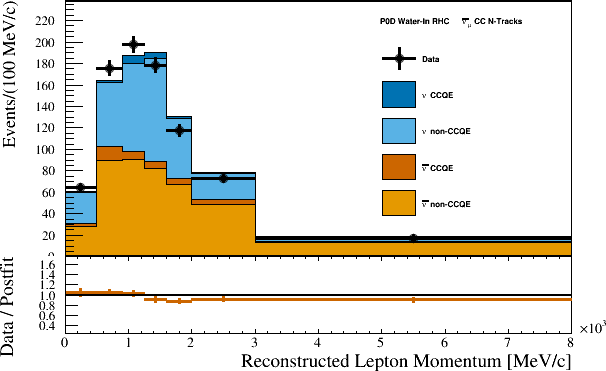
\includegraphics[width=0.45\textwidth,height=0.45\textheight,keepaspectratio]{Chapters/Figures/FitterResults/Postfit/png/P0D_Water_NuMubar_in_Anti_NuMode_CCNTracks_mumom_rxn_postfit}
\par\end{centering}
}\subfloat[$\cos\theta$]{\begin{centering}
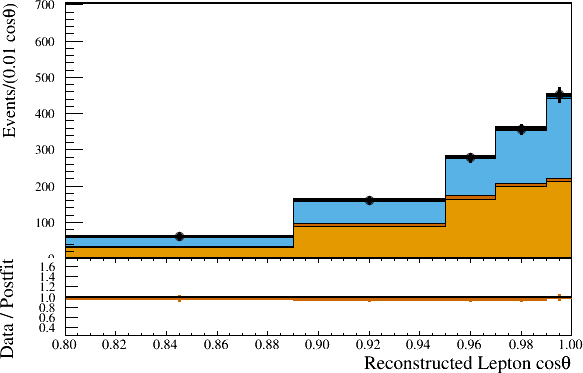
\includegraphics[width=0.45\textwidth,height=0.45\textheight,keepaspectratio]{Chapters/Figures/FitterResults/Postfit/png/P0D_Water_NuMubar_in_Anti_NuMode_CCNTracks_mucostheta_rxn_postfit}
\par\end{centering}
}
\par\end{centering}
\begin{centering}
\subfloat[Momentum-$\cos\theta$]{\begin{centering}
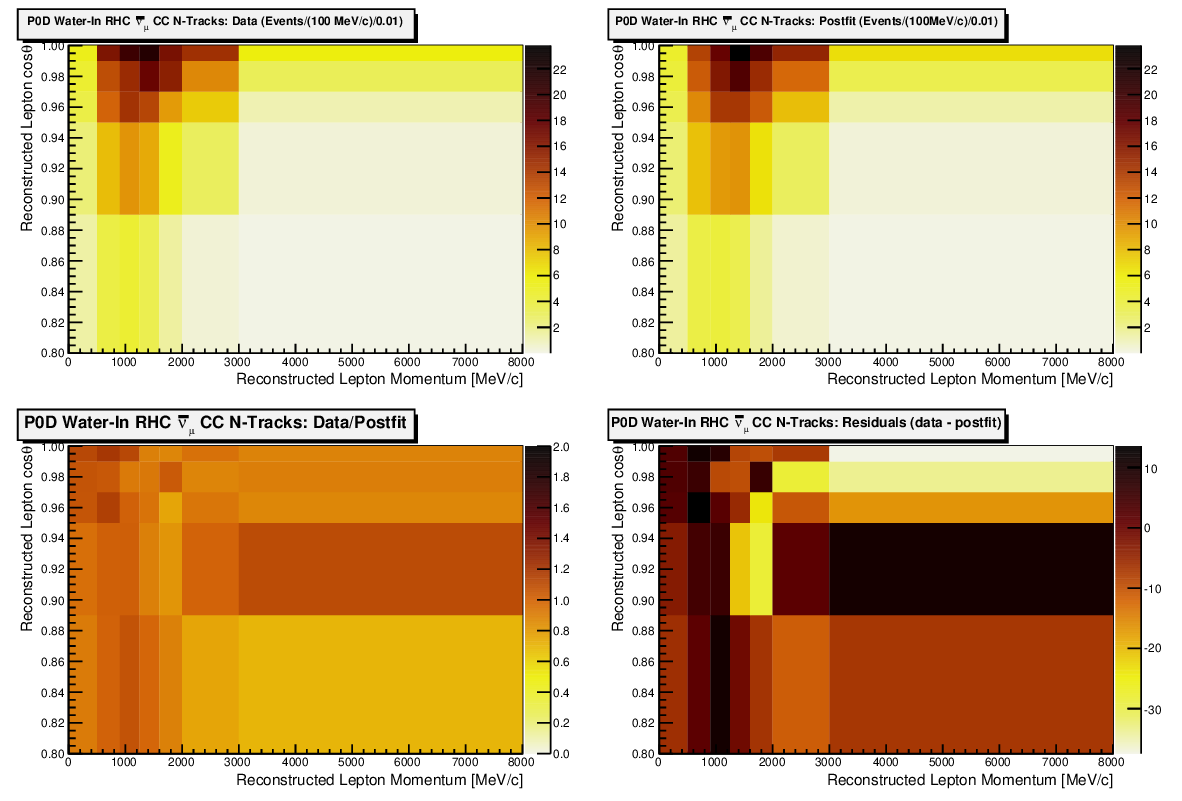
\includegraphics[width=0.99\textwidth]{Chapters/Figures/FitterResults/Postfit/output-3}
\par\end{centering}
}
\par\end{centering}
\caption[Postfit for the Water-In \numubartitle{} in RHC Mode CC 1-Track Sample]{Data and postfit for the $\pod$ Water-In $\protect\numubar$ in RHC
Mode CC N-Tracks sample. Sub-figure (a) shows the momentum one-dimensional
profile in all but the highest momentum fit bin. Sub-figure (b) shows
the $\cos\theta$ one-dimensional profile in all but the highest angle
fit bin. Shown in both (a) and (b) is the ratio between data and the
postfit value. Sub-figure (c) shows a grid of two-dimensional data
and postfit distributions in the same phase space as (a) and (b).
Moving from top-left to bottom-right in (c) is the data, postfit,
data to postfit ratio, and data to postfit difference. \label{fig:Data-and-postfit-wtr-numubarRHCNTrks}
}
\end{figure}

\begin{figure}
\begin{centering}
\subfloat[Momentum in MeV/c]{\begin{centering}
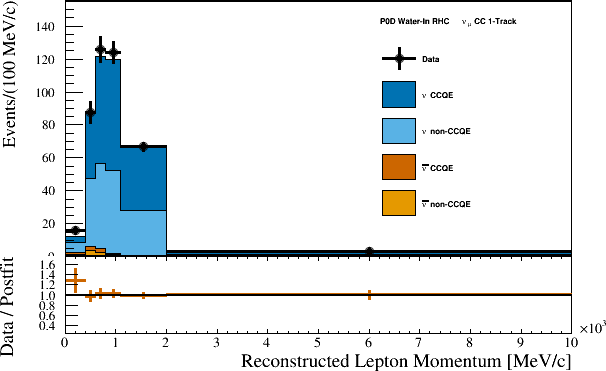
\includegraphics[width=0.45\textwidth,height=0.45\textheight,keepaspectratio]{Chapters/Figures/FitterResults/Postfit/png/P0D_Water_NuMu_Bkg_in_Anti_NuMode_CC1Track_mumom_rxn_postfit}
\par\end{centering}
}\subfloat[$\cos\theta$]{\begin{centering}
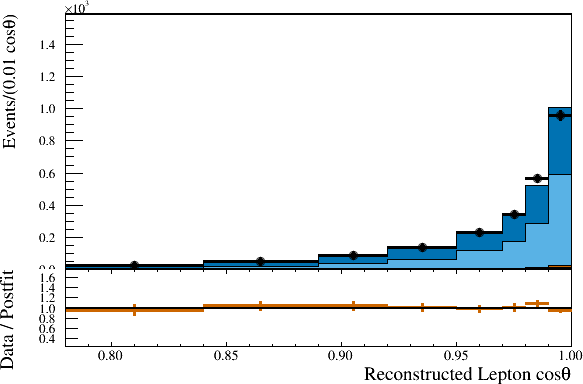
\includegraphics[width=0.45\textwidth,height=0.45\textheight,keepaspectratio]{Chapters/Figures/FitterResults/Postfit/png/P0D_Water_NuMu_Bkg_in_Anti_NuMode_CC1Track_mucostheta_rxn_postfit}
\par\end{centering}
}
\par\end{centering}
\begin{centering}
\subfloat[Momentum-$\cos\theta$]{\begin{centering}
\includegraphics[width=0.99\textwidth]{Chapters/Figures/FitterResults/Postfit/output-4}
\par\end{centering}
}
\par\end{centering}
\caption[Postfit for the Water-In \numutitle{} in RHC Mode CC 1-Track Sample]{Data and postfit for the $\pod$ Water-In $\protect\numu$ in RHC
Mode CC 1-Track sample. Sub-figure (a) shows the momentum one-dimensional
profile in all but the highest momentum fit bin. Sub-figure (b) shows
the $\cos\theta$ one-dimensional profile in all but the highest angle
fit bin. Shown in both (a) and (b) is the ratio between data and the
postfit value. Sub-figure (c) shows a grid of two-dimensional data
and postfit distributions in the same phase space as (a) and (b).
Moving from top-left to bottom-right in (c) is the data, postfit,
data to postfit ratio, and data to postfit difference. \label{fig:Data-and-postfit-wtr-numuRHC1Trk}
}
\end{figure}

\begin{figure}
\begin{centering}
\subfloat[Momentum in MeV/c]{\begin{centering}
\includegraphics[width=0.45\textwidth,height=0.45\textheight,keepaspectratio]{Chapters/Figures/FitterResults/Postfit/png/P0D_Water_NuMu_Bkg_in_Anti_NuMode_CCNTracks_mumom_rxn_postfit}
\par\end{centering}
}\subfloat[$\cos\theta$]{\begin{centering}
\includegraphics[width=0.45\textwidth,height=0.45\textheight,keepaspectratio]{Chapters/Figures/FitterResults/Postfit/png/P0D_Water_NuMu_Bkg_in_Anti_NuMode_CCNTracks_mucostheta_rxn_postfit}
\par\end{centering}
}
\par\end{centering}
\begin{centering}
\subfloat[Momentum-$\cos\theta$]{\begin{centering}
\includegraphics[width=0.99\textwidth]{Chapters/Figures/FitterResults/Postfit/output-5}
\par\end{centering}
}
\par\end{centering}
\caption[Postfit for the Water-In \numutitle{} in RHC Mode CC N-Tracks Sample]{Data and postfit for the $\pod$ Water-In $\protect\numu$ in RHC
Mode CC N-Tracks sample. Sub-figure (a) shows the momentum one-dimensional
profile in all but the highest momentum fit bin. Sub-figure (b) shows
the $\cos\theta$ one-dimensional profile in all but the highest angle
fit bin. Shown in both (a) and (b) is the ratio between data and the
postfit value. Sub-figure (c) shows a grid of two-dimensional data
and postfit distributions in the same phase space as (a) and (b).
Moving from top-left to bottom-right in (c) is the data, postfit,
data to postfit ratio, and data to postfit difference. \label{fig:Data-and-postfit-wtr-numuRHCNTrks}
}
\end{figure}

\begin{figure}
\begin{centering}
\subfloat[Momentum in MeV/c]{\begin{centering}
\includegraphics[width=0.45\textwidth,height=0.45\textheight,keepaspectratio]{Chapters/Figures/FitterResults/Postfit/png/P0D_Air_NuMu_CC1Track_mumom_rxn_postfit}
\par\end{centering}
}\subfloat[$\cos\theta$]{\begin{centering}
\includegraphics[width=0.45\textwidth,height=0.45\textheight,keepaspectratio]{Chapters/Figures/FitterResults/Postfit/png/P0D_Air_NuMu_CC1Track_mucostheta_rxn_postfit}
\par\end{centering}
}
\par\end{centering}
\begin{centering}
\subfloat[Momentum-$\cos\theta$]{\begin{centering}
\includegraphics[width=0.99\textwidth]{Chapters/Figures/FitterResults/Postfit/output-6}
\par\end{centering}
}
\par\end{centering}
\caption[Postfit for the Water-Out \numutitle{} in FHC Mode CC 1-Track Sample]{Data and postfit for the $\pod$ Water-Out $\protect\numu$ in FHC
Mode CC 1-Track sample. Sub-figure (a) shows the momentum one-dimensional
profile in all but the highest momentum fit bin. Sub-figure (b) shows
the $\cos\theta$ one-dimensional profile in all but the highest angle
fit bin. Shown in both (a) and (b) is the ratio between data and the
postfit value. Sub-figure (c) shows a grid of two-dimensional data
and postfit distributions in the same phase space as (a) and (b).
Moving from top-left to bottom-right in (c) is the data, postfit,
data to postfit ratio, and data to postfit difference. \label{fig:Data-and-postfit-air-numu1Trk}
}
\end{figure}

\begin{figure}
\begin{centering}
\subfloat[Momentum in MeV/c]{\begin{centering}
\includegraphics[width=0.45\textwidth,height=0.45\textheight,keepaspectratio]{Chapters/Figures/FitterResults/Postfit/png/P0D_Air_NuMu_CCNTracks_mumom_rxn_postfit}
\par\end{centering}
}\subfloat[$\cos\theta$]{\begin{centering}
\includegraphics[width=0.45\textwidth,height=0.45\textheight,keepaspectratio]{Chapters/Figures/FitterResults/Postfit/png/P0D_Air_NuMu_CCNTracks_mucostheta_rxn_postfit}
\par\end{centering}
}
\par\end{centering}
\begin{centering}
\subfloat[Momentum-$\cos\theta$]{\begin{centering}
\includegraphics[width=0.99\textwidth]{Chapters/Figures/FitterResults/Postfit/output-7}
\par\end{centering}
}
\par\end{centering}
\caption[Postfit for the Water-Out \numutitle{} in FHC Mode CC N-Tracks Sample]{Data and postfit for the $\pod$ Water-Out $\protect\numu$ in FHC
Mode CC N-Tracks sample. Sub-figure (a) shows the momentum one-dimensional
profile in all but the highest momentum fit bin. Sub-figure (b) shows
the $\cos\theta$ one-dimensional profile in all but the highest angle
fit bin. Shown in both (a) and (b) is the ratio between data and the
postfit value. Sub-figure (c) shows a grid of two-dimensional data
and postfit distributions in the same phase space as (a) and (b).
Moving from top-left to bottom-right in (c) is the data, postfit,
data to postfit ratio, and data to postfit difference. \label{fig:Data-and-postfit-air-numuNTrks}
}
\end{figure}

\begin{figure}
\begin{centering}
\subfloat[Momentum in MeV/c]{\begin{centering}
\includegraphics[width=0.45\textwidth,height=0.45\textheight,keepaspectratio]{Chapters/Figures/FitterResults/Postfit/png/P0D_Air_NuMubar_in_Anti_NuMode_CC1Track_mumom_rxn_postfit}
\par\end{centering}
}\subfloat[$\cos\theta$]{\begin{centering}
\includegraphics[width=0.45\textwidth,height=0.45\textheight,keepaspectratio]{Chapters/Figures/FitterResults/Postfit/png/P0D_Air_NuMubar_in_Anti_NuMode_CC1Track_mucostheta_rxn_postfit}
\par\end{centering}
}
\par\end{centering}
\begin{centering}
\subfloat[Momentum-$\cos\theta$]{\begin{centering}
\includegraphics[width=0.99\textwidth]{Chapters/Figures/FitterResults/Postfit/output-8}
\par\end{centering}
}
\par\end{centering}
\caption[Postfit for the Water-Out \numubartitle{} in RHC Mode CC 1-Track
Sample]{Data and postfit for the $\pod$ Water-Out $\protect\numubar$ in
RHC Mode CC 1-Track sample. Sub-figure (a) shows the momentum one-dimensional
profile in all but the highest momentum fit bin. Sub-figure (b) shows
the $\cos\theta$ one-dimensional profile in all but the highest angle
fit bin. Shown in both (a) and (b) is the ratio between data and the
postfit value. Sub-figure (c) shows a grid of two-dimensional data
and postfit distributions in the same phase space as (a) and (b).
Moving from top-left to bottom-right in (c) is the data, postfit,
data to postfit ratio, and data to postfit difference. \label{fig:Data-and-postfit-air-numubarRHC1Trk}
}
\end{figure}

\begin{figure}
\begin{centering}
\subfloat[Momentum in MeV/c]{\begin{centering}
\includegraphics[width=0.45\textwidth,height=0.45\textheight,keepaspectratio]{Chapters/Figures/FitterResults/Postfit/png/P0D_Air_NuMubar_in_Anti_NuMode_CCNTracks_mumom_rxn_postfit}
\par\end{centering}
}\subfloat[$\cos\theta$]{\begin{centering}
\includegraphics[width=0.45\textwidth,height=0.45\textheight,keepaspectratio]{Chapters/Figures/FitterResults/Postfit/png/P0D_Air_NuMubar_in_Anti_NuMode_CCNTracks_mucostheta_rxn_postfit}
\par\end{centering}
}
\par\end{centering}
\begin{centering}
\subfloat[Momentum-$\cos\theta$]{\begin{centering}
\includegraphics[width=0.99\textwidth]{Chapters/Figures/FitterResults/Postfit/output-9}
\par\end{centering}
}
\par\end{centering}
\caption[Postfit for the Water-Out \numubartitle{} in RHC Mode CC N-Tracks
Sample]{Data and postfit for the $\pod$ Water-Out $\protect\numubar$ in
RHC Mode CC N-Tracks sample. Sub-figure (a) shows the momentum one-dimensional
profile in all but the highest momentum fit bin. Sub-figure (b) shows
the $\cos\theta$ one-dimensional profile in all but the highest angle
fit bin. Shown in both (a) and (b) is the ratio between data and the
postfit value. Sub-figure (c) shows a grid of two-dimensional data
and postfit distributions in the same phase space as (a) and (b).
Moving from top-left to bottom-right in (c) is the data, postfit,
data to postfit ratio, and data to postfit difference. \label{fig:Data-and-postfit-air-numubarRHCNTrks}
}
\end{figure}

\begin{figure}
\begin{centering}
\subfloat[Momentum in MeV/c]{\begin{centering}
\includegraphics[width=0.45\textwidth,height=0.45\textheight,keepaspectratio]{Chapters/Figures/FitterResults/Postfit/png/P0D_Air_NuMu_Bkg_in_Anti_NuMode_CC1Track_mumom_rxn_postfit}
\par\end{centering}
}\subfloat[$\cos\theta$]{\begin{centering}
\includegraphics[width=0.45\textwidth,height=0.45\textheight,keepaspectratio]{Chapters/Figures/FitterResults/Postfit/png/P0D_Air_NuMu_Bkg_in_Anti_NuMode_CC1Track_mucostheta_rxn_postfit}
\par\end{centering}
}
\par\end{centering}
\begin{centering}
\subfloat[Momentum-$\cos\theta$]{\begin{centering}
\includegraphics[width=0.99\textwidth]{Chapters/Figures/FitterResults/Postfit/output-10}
\par\end{centering}
}
\par\end{centering}
\caption[Postfit for the Water-Out \numutitle{} in RHC Mode CC 1-Track Sample]{Data and postfit for the $\pod$ Water-Out $\protect\numu$ in RHC
Mode CC 1-Track sample. Sub-figure (a) shows the momentum one-dimensional
profile in all but the highest momentum fit bin. Sub-figure (b) shows
the $\cos\theta$ one-dimensional profile in all but the highest angle
fit bin. Shown in both (a) and (b) is the ratio between data and the
postfit value. Sub-figure (c) shows a grid of two-dimensional data
and postfit distributions in the same phase space as (a) and (b).
Moving from top-left to bottom-right in (c) is the data, postfit,
data to postfit ratio, and data to postfit difference. \label{fig:Data-and-postfit-air-numuRHC1Trk}
}
\end{figure}

\begin{figure}
\begin{centering}
\subfloat[Momentum in MeV/c]{\begin{centering}
\includegraphics[width=0.45\textwidth,height=0.45\textheight,keepaspectratio]{Chapters/Figures/FitterResults/Postfit/png/P0D_Air_NuMu_Bkg_in_Anti_NuMode_CCNTracks_mumom_rxn_postfit}
\par\end{centering}
}\subfloat[$\cos\theta$]{\begin{centering}
\includegraphics[width=0.45\textwidth,height=0.45\textheight,keepaspectratio]{Chapters/Figures/FitterResults/Postfit/png/P0D_Air_NuMu_Bkg_in_Anti_NuMode_CCNTracks_mucostheta_rxn_postfit}
\par\end{centering}
}
\par\end{centering}
\begin{centering}
\subfloat[Momentum-$\cos\theta$]{\begin{centering}
\includegraphics[width=0.99\textwidth]{Chapters/Figures/FitterResults/Postfit/output-11}
\par\end{centering}
}
\par\end{centering}
\caption[Postfit for the Water-Out \numutitle{} in RHC Mode CC N-Tracks Sample]{Data and postfit for the $\pod$ Water-Out $\protect\numu$ in RHC
Mode CC N-Tracks sample. Sub-figure (a) shows the momentum one-dimensional
profile in all but the highest momentum fit bin. Sub-figure (b) shows
the $\cos\theta$ one-dimensional profile in all but the highest angle
fit bin. Shown in both (a) and (b) is the ratio between data and the
postfit value. Sub-figure (c) shows a grid of two-dimensional data
and postfit distributions in the same phase space as (a) and (b).
Moving from top-left to bottom-right in (c) is the data, postfit,
data to postfit ratio, and data to postfit difference. \label{fig:Data-and-postfit-air-numuRHCNTrks}
}
\end{figure}

Now that we have examined the postfit samples and seen that the prediction
has indeed changed, we can proceed to look at the parameter values.

\subsection{Parameter Value and Correlation Comparisons}

The postfit parameters from the $\pod$-only BANFF fit are shown in
\prettyref{fig:Postfit-ND280-flux} through \prettyref{fig:Prefit-and-postfit-bin-normalization}.
A complete listing of the prefit and postfit values is given in Appendix
\prettyref{app:PostfitParameters}. Additionally, a comparison is
made between the $\pod$-only results with that of the FGD-only results.
It must be stated that while the $\pod$-only and FGD-only fits are
using the same 2017 canonical cross section parameterization, the
analyses had different POT exposures. This $\pod$-only analysis fit
uses run periods $2-8$, or about $11.5\times10^{20}$ $\left(6.23\times10^{20}\right)$
POT in FHC (RHC) mode. The FGD-only fit uses runs $2-6$, or about
$5.81\times10^{20}$ $\left(2.84\times10^{20}\right)$ POT in FHC
(RHC) modes. So the $\pod$-only fit has an additional statistical
advantage. This does not affect the actual fitting procedure since
the POT weights scale the MC prediction to the data.

In order to understand how the two analyses compare to each other
in terms of sensitivity to the flux and cross section parameters,
we need to examine each detector's integrated mass-luminosity. The
number of incident neutrinos crossing either the FGD or $\pod$ detector
is the product of its respective fiducial mass and POT exposure. While
the $\pod$ has much more mass, the water-in and water-out modes are
mutually exclusive, resulting in a reduced aggregate POT exposure
as compared to each static FGD for each water-in and water-out running
periods. Also since the FGD2 has a larger water mass fraction compared
to the $\pod$ water-in mode, the expected number of neutrino-oxygen
interaction events are very similar. The comparative advantage of
the $\pod$-only data lies in the number of neutrino-carbon events,
which is about 10 times greater than the FGD. These numbers and more
are tabulated in \prettyref{tab:Neutrino-exposure-P0DFGD}.

\begin{landscape}%

\begin{table}
\caption[Neutrino-Nucleon Exposure on Target Elements]{Neutrino-nucleon exposure on target elements in the $\pod$-only and
FGD-only analyses. The FGD1 and FGD2 masses were calculated using
the following sources\cite{Amaudruz:2012agx,Longhin2016,Lodovico2017}.
The $\pod$ mass was taken from the following source\cite{Schwehr2018}.
The other mass elements include hydrogen, copper, and heavier elements.\label{tab:Neutrino-exposure-P0DFGD}}

\centering{}%
\begin{tabular}{ccccccccccc}
\toprule 
\multirow{2}{*}{Detector} & \multicolumn{4}{c}{Fiducial volume mass} & \multicolumn{2}{c}{POT $\left(10^{20}\right)$} & kg POT & \multicolumn{3}{c}{$\pod$-to-FGD (kg POT)}\tabularnewline
 & (kg) & \ce{^{12}C} (\%) & \ce{^{16}O} (\%) & other (\%) & FHC & RHC & $\left(10^{24}\right)$ & \ce{^{12}C} & \ce{^{16}O} & other\tabularnewline
\midrule
\midrule 
$\pod$ Water-out & 3570 & 70 & 0.67 & 19.33 & 7.872 & - & 2.81 & \multirow{2}{*}{3.99} & \multirow{2}{*}{-} & \multirow{2}{*}{9.21}\tabularnewline
FGD1 & 985 & 86 & 3.7 & 10.3 & 5.81 & - & 0.572 &  &  & \tabularnewline
\midrule 
$\pod$ Water-In & 5470 & 45 & 30 & 25 & 3.657 & - & 2.00 & \multirow{2}{*}{10.63} & \multirow{2}{*}{1.43} & \multirow{2}{*}{8.05}\tabularnewline
FGD2 & 972 & 15 & 74 & 11 & 5.81 & - & 0.565 &  &  & \tabularnewline
\midrule 
$\pod$ Water-out & 3570 & 70 & 0.67 & 19.33 & - & 3.382 & 1.207 & \multirow{2}{*}{3.513} & \multirow{2}{*}{-} & \multirow{2}{*}{8.10}\tabularnewline
FGD1 & 985 & 86 & 3.7 & 10.3 & - & 2.84 & 0.280 &  &  & \tabularnewline
\midrule 
$\pod$ Water-In & 5470 & 45 & 30 & 25 & - & 2.852 & 1.56 & \multirow{2}{*}{16.9} & \multirow{2}{*}{2.29} & \multirow{2}{*}{12.8}\tabularnewline
FGD2 & 972 & 15 & 74 & 11 & - & 2.84 & 0.276 &  &  & \tabularnewline
\bottomrule
\end{tabular}
\end{table}

\end{landscape}%

There is good agreement between the $\pod$-only and FGD-only BANFF
flux parameter values. The flux parameters in both fits follow the
same shape trends, but with the $\pod$-only fit parameters having
a higher expectation comparatively. Also, the magnitude of the flux
uncertainties is similar between the two, which suggests that the
two configurations are statistically similar.

If we examine the bin normalization parameters for the $\pod$-only
fit in \prettyref{fig:Prefit-and-postfit-bin-normalization}, they
are suggesting a reduction in the event rate across most bins. This
high flux, low bin normalization result is likely due to the anticorrelated
relationship between them as indicated in the correlation matrix shown
in \prettyref{fig:Postfit-correlation-matrix}. This has been observed
in previous BANFF analyses. Interestingly, the results of the principal
components analysis on the bin normalizations in Section \ref{subsec:Bin-Normalization-Parameters}
are observed here as well. The analysis predicted most of the parameters
would shift in unison, and we see that trend largely replicated in
the postfit values. This indicates that we can possibly reduce the
number of bin normalizations and still obtain a similar postfit result.

The cross section parameters are also quite similar between the two
fits, with some larger uncertainties in the $\pod$-only result. The
CCQE and BeRPA parameters are in very good agreement with both preferring
a significant increase in the BeRPA $B$ scale parameter. There is
tension in the fits with the $M_{A}^{\text{Res}}$ parameter which
is not currently understood. However, if the difference in the postfit
parameters is distributed according to a chi-squared distribution,
then this deviation is not unexpected. 

A couple of interesting features are observed in the 2p2h parameters.
Firstly is the 2p2h $\nu$ normalization on carbon which is about
two-times larger in the $\pod$-only fit than the FGD-only fit. This
normalization result is currently an unknown phenomenon. It could
be explained by the fact that the $\pod$ has nearly twice as much
non-carbon and non-oxygen elements, which is mostly brass, by mass
fraction as in the FGD (see \prettyref{tab:Neutrino-exposure-P0DFGD}).
The second feature involves the 2p2h shape parameters, \textit{both
of which have postfit values at the physical limit of +1}, or +2 as
shown graphically in \prettyref{fig:Postfit-Xsec}. This predicts
that the 2p2h interaction has no nucleon-nucleon correlation mode
and is only due to the pionless-Delta-decay mode. This result is an
artifact of the cross section parameterization that is also shared
with the FGD result. This issue has been addressed in the latest cross
section parameterization and BANFF analysis\cite{Morrison2019}.

To provide an uncertainty on those shape parameters, even though they
are situated at a discontinuity in the derivative, a ``mirrored''
spline was implemented as shown in \prettyref{fig:The-mirrored-spline}.
The mirrored spline was shown by the BANFF group to not affect the
postfit results while providing a calculable uncertainty in MINUIT
for the Hessian matrix\cite{Bienstock2017}. To further investigate
the impact of a mirrored spline, the oscillation analysis group used
the same splines in the Bayesian analysis, which uses a Markov chain
Monte Carlo method to explore the parameter space. The Bayesian analysis
observed some small relative changes in the 2p2h and $I_{1/2}$ background
normalizations and BeRPA $E$ root-mean-square using the mirrored
spline. However, the parameters that received the largest shifts are
already poorly constrained by the ND280 data, and so they have a minuscule
effect on the fit.

The postfit correlations are shown in \prettyref{fig:Postfit-correlation-matrix}.
The full matrix shows large anticorrelations between the systematic
parameters sets. Largest in magnitude are the flux and cross section
parameters. To better see the correlations for those sets, they are
zoomed into on \prettyref{fig:Prefit-and-post-fluxxsec-correlation}.
For only the cross section parameters, the correlations are shown
in \prettyref{fig:Prefit-and-post-xsec-correlation}.

\begin{figure}
\begin{centering}
\subfloat[$\protect\numu$ in FHC Flux]{\begin{centering}
\includegraphics[width=0.45\textwidth,height=0.18\textheight,keepaspectratio]{Chapters/Figures/FitterResults/P0DvsTN324/output_nd5_numode_numu_bins}
\par\end{centering}
}\subfloat[$\protect\numubar$ in FHC Flux]{\begin{centering}
\includegraphics[width=0.45\textwidth,height=0.18\textheight,keepaspectratio]{Chapters/Figures/FitterResults/P0DvsTN324/output_nd5_numode_numub_bins}
\par\end{centering}
}
\par\end{centering}
\begin{centering}
\subfloat[$\protect\nue$ in FHC Flux]{\begin{centering}
\includegraphics[width=0.45\textwidth,height=0.18\textheight,keepaspectratio]{Chapters/Figures/FitterResults/P0DvsTN324/output_nd5_numode_nue_bins}
\par\end{centering}
}\subfloat[$\protect\nuebar$ in FHC Flux]{\begin{centering}
\includegraphics[width=0.45\textwidth,height=0.18\textheight,keepaspectratio]{Chapters/Figures/FitterResults/P0DvsTN324/output_nd5_numode_nueb_bins}
\par\end{centering}
}
\par\end{centering}
\begin{centering}
\subfloat[$\protect\numu$ in RHC Flux]{\begin{centering}
\includegraphics[width=0.45\textwidth,height=0.18\textheight,keepaspectratio]{Chapters/Figures/FitterResults/P0DvsTN324/output_nd5_anumode_numu_bins}
\par\end{centering}
}\subfloat[$\protect\numubar$ in RHC Flux]{\begin{centering}
\includegraphics[width=0.45\textwidth,height=0.18\textheight,keepaspectratio]{Chapters/Figures/FitterResults/P0DvsTN324/output_nd5_anumode_numub_bins}
\par\end{centering}
}
\par\end{centering}
\begin{centering}
\subfloat[$\protect\nue$ in RHC Flux]{\begin{centering}
\includegraphics[width=0.45\textwidth,height=0.18\textheight,keepaspectratio]{Chapters/Figures/FitterResults/P0DvsTN324/output_nd5_anumode_nue_bins}
\par\end{centering}
}\subfloat[$\protect\nuebar$ in RHC Flux]{\begin{centering}
\includegraphics[width=0.45\textwidth,height=0.18\textheight,keepaspectratio]{Chapters/Figures/FitterResults/P0DvsTN324/output_nd5_anumode_nueb_bins}
\par\end{centering}
}
\par\end{centering}
\caption[Postfit ND280 Flux Parameters for the \podtitle{}-only BANFF Fit]{Postfit ND280 flux parameters for the $\pod$-only (green) and FGD-only
(blue) BANFF fit as functions of neutrino energy. The energy that
maximizes the $\protect\numu\rightarrow\protect\nue$ oscillation
$\left(0.6\text{ GeV}\right)$ is shown with a dashed, black line.\label{fig:Postfit-ND280-flux}}
\end{figure}

\begin{figure}
\begin{centering}
\subfloat[$\protect\numu$ in FHC Flux]{\begin{centering}
\includegraphics[width=0.45\textwidth,height=0.18\textheight,keepaspectratio]{Chapters/Figures/FitterResults/P0DvsTN324/output_sk_numode_numu_bins}
\par\end{centering}
}\subfloat[$\protect\numubar$ in FHC Flux]{\begin{centering}
\includegraphics[width=0.45\textwidth,height=0.18\textheight,keepaspectratio]{Chapters/Figures/FitterResults/P0DvsTN324/output_sk_numode_numub_bins}
\par\end{centering}
}
\par\end{centering}
\begin{centering}
\subfloat[$\protect\nue$ in FHC Flux]{\begin{centering}
\includegraphics[width=0.45\textwidth,height=0.18\textheight,keepaspectratio]{Chapters/Figures/FitterResults/P0DvsTN324/output_sk_numode_nue_bins}
\par\end{centering}
}\subfloat[$\protect\nuebar$ in FHC Flux]{\begin{centering}
\includegraphics[width=0.45\textwidth,height=0.18\textheight,keepaspectratio]{Chapters/Figures/FitterResults/P0DvsTN324/output_sk_numode_nueb_bins}
\par\end{centering}
}
\par\end{centering}
\begin{centering}
\subfloat[$\protect\numu$ in RHC Flux]{\begin{centering}
\includegraphics[width=0.45\textwidth,height=0.18\textheight,keepaspectratio]{Chapters/Figures/FitterResults/P0DvsTN324/output_sk_anumode_numu_bins}
\par\end{centering}
}\subfloat[$\protect\numubar$ in RHC Flux]{\begin{centering}
\includegraphics[width=0.45\textwidth,height=0.18\textheight,keepaspectratio]{Chapters/Figures/FitterResults/P0DvsTN324/output_sk_anumode_numub_bins}
\par\end{centering}
}
\par\end{centering}
\begin{centering}
\subfloat[$\protect\nue$ in RHC Flux]{\begin{centering}
\includegraphics[width=0.45\textwidth,height=0.18\textheight,keepaspectratio]{Chapters/Figures/FitterResults/P0DvsTN324/output_sk_anumode_nue_bins}
\par\end{centering}
}\subfloat[$\protect\nuebar$ in RHC Flux]{\begin{centering}
\includegraphics[width=0.45\textwidth,height=0.18\textheight,keepaspectratio]{Chapters/Figures/FitterResults/P0DvsTN324/output_sk_anumode_nueb_bins}
\par\end{centering}
}
\par\end{centering}
\caption[Postfit SK Flux Parameters for the \podtitle{}-only BANFF Fit]{Postfit SK flux parameters for the $\pod$-only (green) and FGD-only
(blue) BANFF fit as functions of neutrino energy. The energy that
maximizes the $\protect\numu\rightarrow\protect\nue$ oscillation
$\left(0.6\text{ GeV}\right)$ is shown with a dashed, black line.\label{fig:Postfit-SK-flux}}
\end{figure}

\begin{figure}
\begin{centering}
\subfloat[CC-$0\pi$ Parameters]{\begin{centering}
\includegraphics[height=0.35\textheight]{Chapters/Figures/FitterResults/P0DvsTN324/output_CC-QE_and_2p2h_parameters}
\par\end{centering}
}
\par\end{centering}
\begin{centering}
\subfloat[BeRPA Parameters]{\begin{centering}
\includegraphics[width=0.45\textwidth]{Chapters/Figures/FitterResults/P0DvsTN324/output_BeRPA_parameters}
\par\end{centering}
}\subfloat[CC-$1\pi$ Parameters]{\begin{centering}
\includegraphics[width=0.45\textwidth]{Chapters/Figures/FitterResults/P0DvsTN324/output_CC-1#pi_parameters}
\par\end{centering}
}
\par\end{centering}
\begin{centering}
\subfloat[FSI Parameters]{\begin{centering}
\includegraphics[width=0.45\textwidth]{Chapters/Figures/FitterResults/P0DvsTN324/output_FSI_parameters}
\par\end{centering}
}\subfloat[CC-Other and NC-Other Parameters]{\begin{centering}
\includegraphics[width=0.45\textwidth]{Chapters/Figures/FitterResults/P0DvsTN324/output_Other}
\par\end{centering}
}
\par\end{centering}
\caption[Postfit Cross Section Parameters for the $\pod$-only BANFF Fit]{Postfit cross section parameters for the $\pod$-only (green) and
FGD-only (blue) BANFF fit. In these figures, all shape and scale factor
parameters are adjusted to 1 to provide a consistent graphical representation
of all fit parameters. Shape parameters always have a prefit value
of 0. Parameters without prefit uncertainties had a flat prior applied
to them and an asterisk ({*}) represents a fixed parameter. \label{fig:Postfit-Xsec}}
\end{figure}

\begin{figure}
\begin{centering}
\subfloat[Water-In]{\begin{centering}
\includegraphics[width=0.95\textwidth,height=0.425\textheight,keepaspectratio]{Chapters/Figures/FitterResults/Postfit/output_P0D_Water-In_Bin_Norm\lyxdot }
\par\end{centering}
}
\par\end{centering}
\begin{centering}
\subfloat[Water-Out]{\begin{centering}
\includegraphics[width=0.95\textwidth,height=0.425\textheight,keepaspectratio]{Chapters/Figures/FitterResults/Postfit/output_P0D_Water-Out_Bin_Norm\lyxdot }
\par\end{centering}
}
\par\end{centering}
\caption[Prefit and Postfit Bin Normalization Parameters]{Prefit and postfit $\pod$ bin normalization parameters.\label{fig:Prefit-and-postfit-bin-normalization}}
\end{figure}

\begin{figure}
\begin{centering}
\includegraphics[width=0.6\textwidth]{Chapters/Figures/FitterResults/2p2hShapeCSpline}
\par\end{centering}
\caption[The 2p2h Shape Mirrored Spline]{The ``mirrored'' spline for a single event. The spline represents
an event weight and variations from the prefit value of 0 alters the
event weight. The 2p2h shape splines are mirrored about the value
of +1 to provide an uncertainty in the postfit result.\label{fig:The-mirrored-spline}}
\end{figure}

\begin{figure}
\begin{centering}
\includegraphics[width=0.95\textwidth]{Chapters/Figures/FitterResults/Postfit/covariance/corr_post}
\par\end{centering}
\caption[Postfit Correlation Matrix]{Postfit correlation matrix. The first 100 parameters are the flux
parameters with the first 50 corresponding to ND280 and the last 50
with Super-K. Between 100 and 561 are the bin normalization parameters.
The last 31 are the cross section parameters.\label{fig:Postfit-correlation-matrix}}
\end{figure}

\begin{figure}
\begin{centering}
\subfloat[Prefit flux and cross sections correlations]{\begin{centering}
\includegraphics[height=0.4\textheight]{Chapters/Figures/FitterResults/Postfit/covariance/corr_flux_xsec_pref}
\par\end{centering}
\centering{}}
\par\end{centering}
\begin{centering}
\subfloat[Postfit flux and cross section correlations]{\begin{centering}
\includegraphics[height=0.4\textheight]{Chapters/Figures/FitterResults/Postfit/covariance/corr_flux_xsec}
\par\end{centering}
\centering{}}
\par\end{centering}
\caption[Prefit and Post Flux and Cross Section Parameter Correlations]{Prefit and post flux and cross section parameter correlations. In
(a) and (b), the prefit and postfit, respectively, correlation matrices
for the flux and cross section parameters are shown. The first 50
parameters correspond to the ND280 flux with the last 50 with the
SK flux. The final 31 parameters are for the cross section.\label{fig:Prefit-and-post-fluxxsec-correlation}}
\end{figure}

\begin{figure}
\begin{centering}
\includegraphics[width=0.98\textwidth]{Chapters/Figures/FitterResults/Postfit/covariance/corr_xsec}
\par\end{centering}
\caption[Prefit and Post Flux and Cross Section Parameter Correlations]{Postfit cross section correlation matrix\label{fig:Prefit-and-post-xsec-correlation}}
\end{figure}


\subsection{Receiver Operating Characteristic}

To demonstrate the differences between the $\pod$ and FGD parameter
estimates, receiver operating characteristic (ROC) curves are provided
in Appendix \prettyref{app:Receiver-Operating-Characteristi}. The
advantage of ROC curves over a p-value calculation is that the differences
between the two fits can be statistically quantified for all parameters.
These curves provide an indication of which fit has better constraints
in parameter space, suggest the limitation of each fit, and provide
guidance for future researchers.

\section{Summary\label{sec:ResultsSummary}}

In this chapter, we have explored the postfit results for the $\pod$-only
data set and compared it against the FGD-only fit. While the FGD-only
data samples have about twice as many more neutrino-oxygen events
than the $\pod$-only data, which helps with sensitivity of the oxygen
cross section parameters, the accumulated neutrino exposures are similar.
Moreover, we observe a good level of agreement between the two fits
with the largest differences observed with less constrained parameters
like those that characterize the 2p2h interaction. We will examine
in the final chapter the differences in the predicted neutrino energy
spectrum at SK using the $\pod$-only and FGD-only postfit results.
